%%%%%%%%%%%%%%%%%%%%%%%%%%%%%%%%%%%%%%%%%
% Short Sectioned Assignment
% LaTeX Template
% Version 1.0 (5/5/12)
%
% This template has been downloaded from:
% http://www.LaTeXTemplates.com
%
% Original author:
% Frits Wenneker (http://www.howtotex.com)
%
% License:
% CC BY-NC-SA 3.0 (http://creativecommons.org/licenses/by-nc-sa/3.0/)
%
% Download template:
% Overleaf (https://www.overleaf.com/8746855dtrgkbkbjjhm)
%
%%%%%%%%%%%%%%%%%%%%%%%%%%%%%%%%%%%%%%%%%

%-------------------------------------------------------------------------------
%	PACKAGES AND OTHER DOCUMENT CONFIGURATIONS
%-------------------------------------------------------------------------------

%\documentclass[paper=a4, fontsize=11pt]{scrartcl} % A4 paper and 11pt font size
%\documentclass[a4paper]{article}
\documentclass[12pt]{article}
%\usepackage[margin=1.25in]{geometry}

%\usepackage[options]{nohyperref}  % This makes hyperref commands do nothing without errors
%\usepackage{url}  % This makes \url work
%\usepackage{hyperref}

\usepackage{graphicx}

%\usepackage[T1]{fontenc} % Use 8-bit encoding that has 256 glyphs
\usepackage[utf8]{inputenc}
%\usepackage{fourier} % Use the Adobe Utopia font for the document - comment this line to return to the LaTeX default
\usepackage[english]{babel} % English language/hyphenation
\usepackage{mathtools,amsmath,amsfonts,amsthm} % Math packages
\usepackage{amssymb}

%\usepackage{lipsum} % Used for inserting dummy 'Lorem ipsum' text into the template

\usepackage{sectsty} % Allows customizing section commands
\allsectionsfont{\centering \normalfont\scshape} % Make all sections centered, the default font and small caps

\usepackage{fancyhdr} % Custom headers and footers
%\pagestyle{fancyplain} % Makes all pages in the document conform to the custom headers and footers
%\fancyhead{} % No page header - if you want one, create it in the same way as the footers below
%\fancyfoot[L]{} % Empty left footer
%\fancyfoot[C]{} % Empty center footer
%\fancyfoot[R]{\thepage} % Page numbering for right footer
\renewcommand{\headrulewidth}{0pt} % Remove header underlines
\renewcommand{\footrulewidth}{0pt} % Remove footer underlines
\setlength{\headheight}{13.6pt} % Customize the height of the header

\numberwithin{equation}{section} % Number equations within sections (i.e. 1.1, 1.2, 2.1, 2.2 instead of 1, 2, 3, 4)
\numberwithin{figure}{section} % Number figures within sections (i.e. 1.1, 1.2, 2.1, 2.2 instead of 1, 2, 3, 4)
\numberwithin{table}{section} % Number tables within sections (i.e. 1.1, 1.2, 2.1, 2.2 instead of 1, 2, 3, 4)

%\setlength\parindent{0pt} % Removes all indentation from paragraphs - comment this line for an assignment with lots of text
\usepackage{indentfirst} % Indentation for all paragraphs

% Used for definitions:
\usepackage{amsthm}
\theoremstyle{definition}
\newtheorem{definition}{Definition}[section]

% To write algorithms in pseudocode:
\usepackage{algpseudocode}
\usepackage{algorithm}

% Don't use colon in algorithms lines:
\algrenewcommand\alglinenumber[1]{\footnotesize #1}

% Input/Output instead of Require/Ensure in algorithms pseudocode:
\renewcommand{\algorithmicrequire}{\textbf{Input:}}
\renewcommand{\algorithmicensure}{\textbf{Output:}}

% To put images side by side:
\usepackage{subcaption}

% Avoid long sentences to go out of margines:
\usepackage{microtype}

% Use URL and avoid long urls to go out of margins (hyphens):
\usepackage[hyphens]{url}

\usepackage{pgfplots}
\pgfplotsset{compat=1.15}

% Define multiline to avoid unindented long sentences in algorithms:
% (https://tex.stackexchange.com/questions/314023/how-to-indent-a-long-sentence-in-an-algorithm)
\usepackage{tabularx}
\makeatletter
\newcommand{\multiline}[1]{%
  \begin{tabularx}{\dimexpr\linewidth-\ALG@thistlm}[t]{@{}X@{}}
    #1
  \end{tabularx}
}
\makeatother

%-------------------------------------------------------------------------------
%	TITLE SECTION
%-------------------------------------------------------------------------------

\newcommand{\horrule}[1]{\rule{\linewidth}{#1}} % Create horizontal rule command with 1 argument of height

\title{
\normalfont \normalsize
\textsc{Sapienza University of Rome} \\ [25pt] % Your university, school and/or department name(s)
\horrule{0.5pt} \\[0.4cm] % Thin top horizontal rule
\LARGE Vision and Perception \\ % The assignment title
\large Mask R-CNN and Activity Recognition \\
\horrule{2pt} \\[0.5cm] % Thick bottom horizontal rule
}

\author{Ivan Bergonzani, Michele Cipriano,\\Ibis Prevedello, Jean-Pierre Richa} % Your name

\date{\normalsize\today} % Today's date or a custom date

\begin{document}
\sloppy % avoid to make words to go out of margin

\maketitle % Print the title

%-------------------------------------------------------------------------------

\section{Introduction}

The aim of the project is to train a model based on Mask R-CNN\cite{he2017maskrcnn}
using an extended version of COCO that includes the dataset created on Labelbox and use it to train another network
that recognizes activities from videos.
The new dataset consists on a bunch of images that shows the Gymnastic activities
of ActivityNet. All the images have been downloaded from Google using a Python
tool called \texttt{google-images-download}. The idea is to have a working model that
will be used to classify videos that show Gymnastic activities.
This second task is achieved by training a LSTM on the 
frames taken from the videos themselves.

The project has been developed in Python and it has been tested using Google
Compute Engine. The final training of Mask R-CNN has been performed at Alcor lab, while the training of the LSTM
has been performed on a Google Compute Engine instance.

%-------------------------------------------------------------------------------

\section{Mask R-CNN Training}

Mask R-CNN has a set of losses that are used to check the performances of the
classification, the RPN, the regression on the bounding boxes and the instance
segmentation:
\begin{itemize}
    \item \texttt{smooth\_l1\_loss}: the smooth-L1 loss on the classification of the
        objects.
    \item \texttt{rpn\_class\_loss}: the loss on the classification of the
        object contained in the region proposals, they can either be foreground
        if there is an object inside or background otherwise.
    \item \texttt{rpn\_bbox\_loss}: the loss on the bounding box returned by the RPN.
    \item \texttt{mrcnn\_class\_loss}: the loss for the classifier head of Mask
        R-CNN.
    \item \texttt{mrcnn\_bbox\_loss}: the loss for the bounding box refinement
        at the end of the network.
    \item \texttt{mrcnn\_mask\_loss}: the binary cross-entropy loss for the masks.
\end{itemize}

It is possible to see the graphs of these losses using
tensorboard once the
training is complete. The network has been trained for 35
epochs for the first stage, 30 epochs for the second and
15 epochs for the third stage, being able to recognize most
of the objects in the videos. The dataset used has been those
created from LabelBox that is summarized in table
\ref{table:labelbox-masks-summary}. The dataset has been
split in 90\% for the training set and 10\% for the test set.
The network, when using \texttt{DETECTION\_MIN\_CONFIDENCE=0.9},
obtained a number of 127 successes out of 169
labels with a success percentage of \textbf{0.751}.

\begin{table}
	\centering
	\begin{tabular}{*{2}{c}}
		Activity & Labels \\
		\hline
		Doing step aerobics & 268 \\
		Elliptical trainer & 177 \\
		Spinning & 158 \\
		Using parallel bars & 241 \\
		Using the balance beam & 383 \\
		Using the pommel horse & 248 \\
		Using the rowing machine & 290 \\
		Using uneven bars & 253 \\
		\hline
		\textbf{Total} & \textbf{2018}
	\end{tabular}
	\caption{Number of masks segmented in LabelBox for
	    each activity in Gymnastics.}
	\label{table:labelbox-masks-summary}
\end{table}

%-------------------------------------------------------------------------------

\section{Activity Recognition}

Once Mask R-CNN training is complete it is possible to 
use the resulting model to extract features and informations
from the frames of the videos.

To do this, each video has been preprocessed by removing the
first 10\% and the last 10\% of the frames that likely contain
frames that do not contribute to the recognition of the video
(e.g. advertisement). From the remaining part of the video,
40 frames have been extracted uniformly and saved.
Then, each frame has been fed to the Mask R-CNN model obtained
previously. The output masks and the output labels coming
from Mask R-CNN have been
used to build the tensors to be fed to the LSTM. In order
to speed up the training of the activity recognizer, these
data are saved in a separate file so that they can be used 
without going through Mask R-CNN again.

The problem is, hence, reduced to training a LSTM. Multiple
experiments have been performed on the features extracted
from Mask R-CNN, all summarized in table
\ref{table:lstm-experiments}. In particular the trainings
focused on the number of hidden nodes for the LSTM and the
type of features extracted. The number of hidden nodes
varied from 64 to 1024. Three types of datasets have
been created by extracting the features from the videos
contained in the dataset Gymnastics, summarized in table
\ref{table:activity-dataset}.
The dataset Count contains a vector
that counts the number of objects contained in each frame of
each video. The dataset Masks contains a tensor with all the
masks recognized by Mask R-CNN. The dataset Masks+Count
combines the two, with the idea of exploiting both kinds
of data. Each dataset has been split in 80\% for the training
set and 20\% for the test set.

\begin{table}
	\centering
	\begin{tabular}{*{3}{c}}
		Num. & Activity & Videos \\
		\hline
		1 & Doing crunches & 62 \\
		2 & Doing step aerobics & 78 \\
		3 & Elliptical trainer & 79 \\
		4 & Kneeling & 92 \\
		5 & Rope skipping & 101 \\
		6 & Running a marathon & 81 \\
		7 & Spinning & 78 \\
		8 & Tumbling & 61 \\
		9 & Using parallel bars & 100 \\
		10 & Using the balance beam & 105 \\
		11 & Using the pommel horse & 64 \\
		12 & Using the rowing machine & 68 \\
		13 & Using uneven bars & 63 \\
		14 & Zumba & 61 \\
		\hline
		& \textbf{Total} & \textbf{1093}
	\end{tabular}
	\caption{Number of videos for each activity contained in Gymnastics.}
	\label{table:activity-dataset}
\end{table}

The structure of the network is pretty simple. It consists
of a LSTM followed by a dropout layer (with probability 0.2)
that aims to avoid overfitting. The LSTM considers a timestep
of 40 and outputs a softmax over the classes of the videos
contained in Gymnastics. Since the LSTM requires a 1D vector
as input, the masks are vectorized before being fed to the
LSTM itself. This makes the masks to lose the spatiality
of the data, making it harder to train the network.

It is interesting to study how the accuracy and the loss varies
with the epochs changing the type of data that is used to
train the network and the number of hidden nodes in the 
LSTM. More in detail, each neural network is trained
for two stages that differs in the value of the learning
rate and the number of epochs. All the experiments used
a learning rate of $10^{-3}$ for the first stage and $10^{-4}$
for the second stage. The number of epochs have been chosen
so that there is no overfitting in the test set.

Figures \ref{fig:train-accuracy-masks} and
\ref{fig:test-accuracy-masks} show how the accuracy changes 
over the epochs when using only the masks as input of the
network. The networks are able to learn the activities
represented by the videos, achieving a higher accuracy
more quickly on the training set when using a larger number of
hidden nodes. This is somehow reflected also on the test
set, even if the difference is not large as in the training
set. The same thing
applies when using both masks and the count of the objects
in each frame (figures \ref{fig:train-accuracy-masks+count} and
\ref{fig:test-accuracy-masks+count}).
For this second experiment the LSTM manages
to obtain slightly better results in the test set.
When using only the count of the objects (figures
\ref{fig:train-accuracy-count} and
\ref{fig:test-accuracy-count}) the networks manage to perform
better in the test set with respect to the previous two
experiments. Nevertheless it is not able to achieve a high
accuracy in the training set.

Figures \ref{fig:cm_train} and \ref{fig:cm_test} shows 
the confusion matrices obtained when using an LSTM of 512
hidden layers with only the masks of the objects.
Regarding the training set, the main problem of the network
is on the recognition of the activity ``Using parallel
bars'', that is often confused with ``Using the pommel
horse''. On the test set, the network never manages to
classify a video as ``Tumbling''. The reasons for this
behaviour is due in particular to the extraction of the
masks when using Mask R-CNN. Hence, an improvement of
Mask R-CNN would improve the quality of the dataset that would,
in turn, improve the accuracy of the LSTM. Moreover, the
network does not guarantee that it is able to extract
at least one mask for every frame of the video, hence, using
more frames, or selecting better frames for each video would
improve the accuracy of the LSTM, increasing the accuracy of
the activity classification.
This, however, is very expensive from a
computational point of view, since it would require going
through Mask R-CNN more often.

The structure of the network could be improved by considering
the spatial relations of the frames. In fact, since the LSTM
requires an input a 1D vector, all the frames have been
vectorized. One possibility is to replace the LSTM
with a Grid LSTM\cite{Kalchbrenner2015GridLS}, that
accept as input a tensor of any dimension, like in the
case of the frames.

\begin{table}
	\centering
	\begin{tabular}{*{6}{c}}
		Network & Dataset & Stage 1 & Stage 2 & Train Acc. & Test. Acc. \\
		\hline
		LSTM-64 & Count & 250 & 300 & 0.499 & 0.516 \\
		LSTM-128 & Count & 250 & 300 & 0.505 & 0.512 \\
		LSTM-256 & Count & 250 & 300 & 0.525 & \textbf{0.532} \\
		LSTM-512 & Count & 250 & 300 & \textbf{0.619} & 0.488 \\
		LSTM-1024 & Count & 250 & 300 & 0.616 & 0.500 \\
		\hline
		LSTM-64 & Masks & 15 & 50 & 0.735 & 0.391 \\
		LSTM-128 & Masks & 15 & 50 & 0.869 & 0.435 \\
		LSTM-256 & Masks & 15 & 50 & 0.914 & 0.419 \\
		LSTM-512 & Masks & 15 & 50 & \textbf{0.928} & \textbf{0.452} \\
		LSTM-1024 & Masks & 15 & 50 & 0.924 & 0.427 \\
		\hline
		LSTM-64 & Masks+Count & 15 & 50 & 0.706 & 0.419 \\
		LSTM-128 & Masks+Count & 15 & 50 & 0.865 & 0.456 \\
		LSTM-256 & Masks+Count & 15 & 50 & 0.913 & \textbf{0.492} \\
		LSTM-512 & Masks+Count & 15 & 50 & 0.921 & 0.423 \\
		LSTM-1024 & Masks+Count & 15 & 50 & \textbf{0.928} & 0.435 \\
	\end{tabular}
	\caption{The table shows the results of the experiments.
	    Different number of hidden nodes have been tried
	    for the LSTM. All the datasets contain different
	    informations from the frames of the videos:
	    Count represents each frame as a vector containing
	    the number of objects in the frame itself, Masks
	    represents each frame as a semantic map,
	    Masks+Count combines the two. Note that since the
	    LSTM requires a 1D vector as input, all the datasets
	    have been vectorized before being fed to the LSTM.
	    Note that even if the number epochs is higher
	    for the datase Count, it takes less time to train
	    w.r.t. the other two datasets. For example, when
	    using LSTM-512 it takes \textbf{4m59s} on Count and
	    \textbf{16m25s} on Masks on an instance of Google
	    Compute Engine with a Tesla K80.}
    \label{table:lstm-experiments}
\end{table}

\begin{figure}
    \centering
    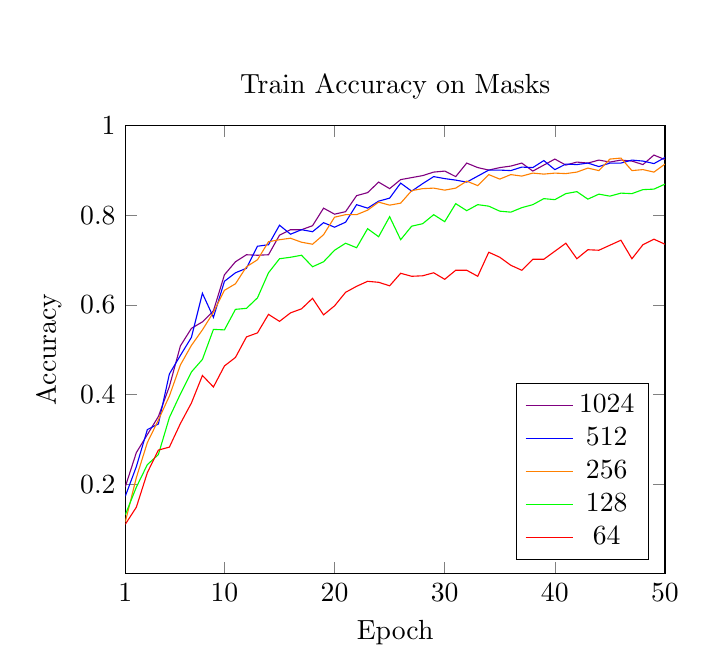
\begin{tikzpicture}
        \begin{axis}[
            title={Train Accuracy on Masks},
            xlabel={Epoch},
            ylabel={Accuracy},
            xmin=1, xmax=50,
            ymin=0, ymax=1,
            xtick={1,10,20,30,40,50},
            ytick={0.2,0.4,0.6,0.8,1.0},
            legend pos=south east,
            %ymajorgrids=true,
            %grid style=dashed,
        ]
         
        \addplot[color=violet]
            coordinates{
                (1, 0.19441340863704681) (2, 0.270391047000885) (3, 0.31061452627182007) (4, 0.35083797574043274) (5, 0.41787710785865784) (6, 0.5083798766136169) (7, 0.5474860072135925) (8, 0.562011182308197) (9, 0.5865921974182129) (10, 0.6670390963554382) (11, 0.6960893869400024) (12, 0.7117318511009216) (13, 0.7106145024299622) (14, 0.7117318511009216) (15, 0.7553072571754456) (16, 0.7675977945327759) (17, 0.7675977945327759) (18, 0.7765362858772278) (19, 0.8156424760818481) (20, 0.8022346496582031) (21, 0.8078212141990662) (22, 0.8435754179954529) (23, 0.8502793312072754) (24, 0.8737429976463318) (25, 0.8592178821563721) (26, 0.8793296217918396) (27, 0.8837988972663879) (28, 0.8882681727409363) (29, 0.8960893750190735) (30, 0.8983240127563477) (31, 0.8860335350036621) (32, 0.916201114654541) (33, 0.9061452746391296) (34, 0.9005586504936218) (35, 0.9061452746391296) (36, 0.9094972014427185) (37, 0.916201114654541) (38, 0.8983240127563477) (39, 0.9117318391799927) (40, 0.9251396656036377) (41, 0.9117318391799927) (42, 0.9184357523918152) (43, 0.916201114654541) (44, 0.9229050278663635) (45, 0.9184357523918152) (46, 0.9229050278663635) (47, 0.9206703901290894) (48, 0.9128491878509521) (49, 0.9340782165527344) (50, 0.9240223169326782) 
            };
            \addlegendentry{1024}
         
        \addplot[color=blue]
            coordinates {
            (1, 0.1731843501329422) (2, 0.23910614848136902) (3, 0.3217877149581909) (4, 0.33407822251319885) (5, 0.4458100497722626) (6, 0.4871508479118347) (7, 0.5273743271827698) (8, 0.6256983280181885) (9, 0.5720670223236084) (10, 0.6525139808654785) (11, 0.6715083718299866) (12, 0.6815642714500427) (13, 0.7307262420654297) (14, 0.7340782284736633) (15, 0.7776536345481873) (16, 0.7575418949127197) (17, 0.7675977945327759) (18, 0.7631285190582275) (19, 0.7832401990890503) (20, 0.7731843590736389) (21, 0.7843575477600098) (22, 0.8234636783599854) (23, 0.8156424760818481) (24, 0.8312849402427673) (25, 0.8379888534545898) (26, 0.8715083599090576) (27, 0.8536312580108643) (28, 0.8703910708427429) (29, 0.8860335350036621) (30, 0.8815642595291138) (31, 0.8782122731208801) (32, 0.8737429976463318) (33, 0.8871508240699768) (34, 0.9005586504936218) (35, 0.9005586504936218) (36, 0.8994413614273071) (37, 0.9072625637054443) (38, 0.9061452746391296) (39, 0.9217877388000488) (40, 0.9016759991645813) (41, 0.9139664769172668) (42, 0.9128491878509521) (43, 0.916201114654541) (44, 0.9083799123764038) (45, 0.916201114654541) (46, 0.916201114654541) (47, 0.9229050278663635) (48, 0.9206703901290894) (49, 0.9150838255882263) (50, 0.9284915924072266)
            };
            \addlegendentry{512}
         
        \addplot[color=orange]
            coordinates{
                (1, 0.11620111763477325) (2, 0.21452513337135315) (3, 0.2927374243736267) (4, 0.34301677346229553) (5, 0.3966480493545532) (6, 0.4659217894077301) (7, 0.5094972252845764) (8, 0.5441340804100037) (9, 0.5832402110099792) (10, 0.632402241230011) (11, 0.6469273567199707) (12, 0.6849161982536316) (13, 0.7005586624145508) (14, 0.7407821416854858) (15, 0.7452514171600342) (16, 0.748603343963623) (17, 0.7396647930145264) (18, 0.735195517539978) (19, 0.756424605846405) (20, 0.7955307364463806) (21, 0.8011173009872437) (22, 0.8011173009872437) (23, 0.8111732006072998) (24, 0.8290503025054932) (25, 0.8223463892936707) (26, 0.826815664768219) (27, 0.8547486066818237) (28, 0.8592178821563721) (29, 0.8603351712226868) (30, 0.8558658957481384) (31, 0.8603351712226868) (32, 0.875977635383606) (33, 0.8659217953681946) (34, 0.8905028104782104) (35, 0.8804469108581543) (36, 0.8905028104782104) (37, 0.8871508240699768) (38, 0.8938547372817993) (39, 0.8916200995445251) (40, 0.8938547372817993) (41, 0.8927374482154846) (42, 0.8960893750190735) (43, 0.9050279259681702) (44, 0.8994413614273071) (45, 0.9251396656036377) (46, 0.9273743033409119) (47, 0.8994413614273071) (48, 0.9016759991645813) (49, 0.8960893750190735) (50, 0.9139664769172668) 
            };
            \addlegendentry{256}
         
         \addplot[color=green]
            coordinates{(1, 0.13184358179569244) (2, 0.19329608976840973) (3, 0.24357542395591736) (4, 0.26592180132865906) (5, 0.34860333800315857) (6, 0.40111732482910156) (7, 0.4502793252468109) (8, 0.47821229696273804) (9, 0.5452513694763184) (10, 0.5441340804100037) (11, 0.5899441242218018) (12, 0.5921787619590759) (13, 0.6156424283981323) (14, 0.6715083718299866) (15, 0.702793300151825) (16, 0.7061452269554138) (17, 0.7106145024299622) (18, 0.6849161982536316) (19, 0.6960893869400024) (20, 0.721787691116333) (21, 0.7374301552772522) (22, 0.7273743152618408) (23, 0.7698323726654053) (24, 0.7519553303718567) (25, 0.7966480255126953) (26, 0.7452514171600342) (27, 0.7754189968109131) (28, 0.7810055613517761) (29, 0.8011173009872437) (30, 0.7854748368263245) (31, 0.8256983160972595) (32, 0.8100558519363403) (33, 0.8234636783599854) (34, 0.8201117515563965) (35, 0.8089385628700256) (36, 0.8067039251327515) (37, 0.8167597651481628) (38, 0.8234636783599854) (39, 0.8368715047836304) (40, 0.8346368670463562) (41, 0.8480446934700012) (42, 0.8525139689445496) (43, 0.8357542157173157) (44, 0.8469273447990417) (45, 0.8424581289291382) (46, 0.8491619825363159) (47, 0.8480446934700012) (48, 0.8569832444190979) (49, 0.8581005334854126) (50, 0.8692737221717834) };
            \addlegendentry{128}
         
         \addplot[color=red]
            coordinates{(1, 0.11061452329158783) (2, 0.14860334992408752) (3, 0.225698322057724) (4, 0.27597764134407043) (5, 0.28268155455589294) (6, 0.33519554138183594) (7, 0.38100558519363403) (8, 0.4424580931663513) (9, 0.41675978899002075) (10, 0.46368715167045593) (11, 0.4826815724372864) (12, 0.5284916162490845) (13, 0.5374301671981812) (14, 0.5787709355354309) (15, 0.5631284713745117) (16, 0.5821229219436646) (17, 0.5910614728927612) (18, 0.6145251393318176) (19, 0.5776536464691162) (20, 0.5977653861045837) (21, 0.6279329657554626) (22, 0.6413407921791077) (23, 0.6525139808654785) (24, 0.6502793431282043) (25, 0.6424580812454224) (26, 0.6703910827636719) (27, 0.6636871695518494) (28, 0.6648044586181641) (29, 0.6715083718299866) (30, 0.6569832563400269) (31, 0.6770949959754944) (32, 0.6770949959754944) (33, 0.6636871695518494) (34, 0.7173184156417847) (35, 0.7061452269554138) (36, 0.6882681846618652) (37, 0.6770949959754944) (38, 0.7016759514808655) (39, 0.7016759514808655) (40, 0.7195530533790588) (41, 0.7374301552772522) (42, 0.702793300151825) (43, 0.7229050397872925) (44, 0.721787691116333) (45, 0.7329608798027039) (46, 0.7441340684890747) (47, 0.702793300151825) (48, 0.7340782284736633) (49, 0.7463687062263489) (50, 0.735195517539978)};
            \addlegendentry{64}
         
        \end{axis}
    \end{tikzpicture}
    \caption{The plot shows the how the train accuracy
        varies for the dataset Masks changing the number
        of hidden nodes in the LSTM.}
    \label{fig:train-accuracy-masks}
\end{figure}

\begin{figure}
    \centering
    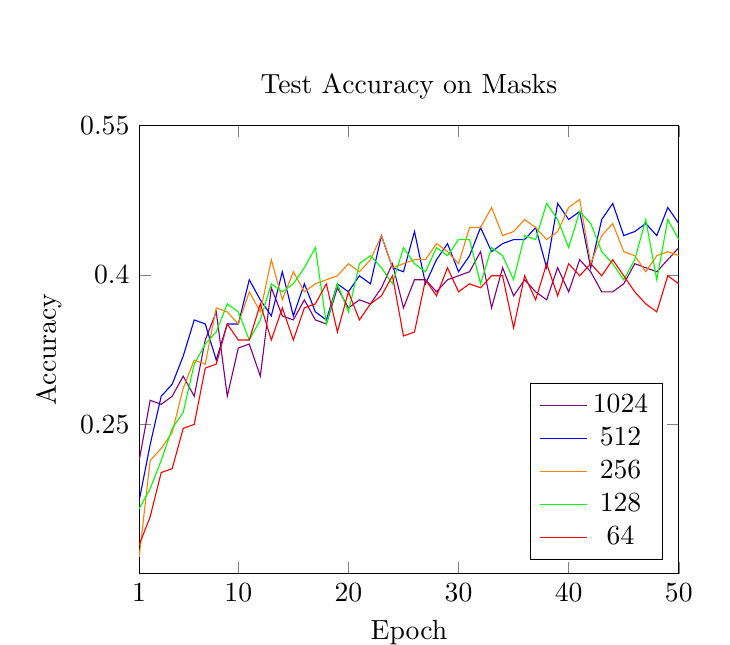
\begin{tikzpicture}
        \begin{axis}[
            title={Test Accuracy on Masks},
            xlabel={Epoch},
            ylabel={Accuracy},
            xmin=1, xmax=50,
            ymin=0.1, ymax=0.55,
            xtick={1,10,20,30,40,50},
            ytick={0.25,0.40,0.55},
            legend pos=south east,
            %ymajorgrids=true,
            %grid style=dashed,
        ]


        \addplot[color=violet]
            coordinates{
                (1, 0.21370968222618103) (2, 0.27419355511665344) (3, 0.27016130089759827) (4, 0.2782258093357086) (5, 0.2983871102333069) (6, 0.2782258093357086) (7, 0.33467742800712585) (8, 0.3629032373428345) (9, 0.2782258093357086) (10, 0.3266128897666931) (11, 0.3306451737880707) (12, 0.2983871102333069) (13, 0.3870967626571655) (14, 0.3588709831237793) (15, 0.35483869910240173) (16, 0.375) (17, 0.35483869910240173) (18, 0.35080644488334656) (19, 0.3870967626571655) (20, 0.36693549156188965) (21, 0.375) (22, 0.3709677457809448) (23, 0.3870967626571655) (24, 0.41129031777381897) (25, 0.36693549156188965) (26, 0.39516130089759827) (27, 0.39516130089759827) (28, 0.38306450843811035) (29, 0.39516130089759827) (30, 0.39919355511665344) (31, 0.4032258093357086) (32, 0.4233870804309845) (33, 0.36693549156188965) (34, 0.4072580635547638) (35, 0.3790322542190552) (36, 0.39516130089759827) (37, 0.38306450843811035) (38, 0.375) (39, 0.4072580635547638) (40, 0.38306450843811035) (41, 0.41532257199287415) (42, 0.4032258093357086) (43, 0.38306450843811035) (44, 0.38306450843811035) (45, 0.3911290466785431) (46, 0.41129031777381897) (47, 0.4072580635547638) (48, 0.4032258093357086) (49, 0.41532257199287415) (50, 0.42741936445236206) 
            };
            \addlegendentry{1024}

        \addplot[color=blue]
            coordinates{
                (1, 0.1733870953321457) (2, 0.22983871400356293) (3, 0.2782258093357086) (4, 0.29032257199287415) (5, 0.31854838132858276) (6, 0.35483869910240173) (7, 0.35080644488334656) (8, 0.3145161271095276) (9, 0.35080644488334656) (10, 0.35080644488334656) (11, 0.39516130089759827) (12, 0.375) (13, 0.3588709533214569) (14, 0.4032258093357086) (15, 0.3588709533214569) (16, 0.3911290466785431) (17, 0.3629032373428345) (18, 0.35483869910240173) (19, 0.3911290168762207) (20, 0.38306450843811035) (21, 0.39919355511665344) (22, 0.3911290466785431) (23, 0.4395161271095276) (24, 0.4072580635547638) (25, 0.4032258093357086) (26, 0.44354838132858276) (27, 0.3911290466785431) (28, 0.41532257199287415) (29, 0.43145161867141724) (30, 0.4032258093357086) (31, 0.4193548262119293) (32, 0.44758063554763794) (33, 0.4233871102333069) (34, 0.43145161867141724) (35, 0.4354838728904724) (36, 0.4354838728904724) (37, 0.44758063554763794) (38, 0.4072580635547638) (39, 0.4717741906642914) (40, 0.4556451737880707) (41, 0.46370968222618103) (42, 0.4072580635547638) (43, 0.4556451737880707) (44, 0.4717741906642914) (45, 0.4395161271095276) (46, 0.44354838132858276) (47, 0.4516128897666931) (48, 0.4395161271095276) (49, 0.4677419364452362) (50, 0.4516128897666931)
            };
            \addlegendentry{512}

        \addplot[color=orange]
            coordinates{
                (1, 0.11693548411130905) (2, 0.21370968222618103) (3, 0.22580644488334656) (4, 0.24193547666072845) (5, 0.28629031777381897) (6, 0.3145161271095276) (7, 0.3104838728904724) (8, 0.36693549156188965) (9, 0.3629032373428345) (10, 0.35080644488334656) (11, 0.38306450843811035) (12, 0.3629032373428345) (13, 0.41532257199287415) (14, 0.375) (15, 0.4032258093357086) (16, 0.38306450843811035) (17, 0.3911290466785431) (18, 0.39516130089759827) (19, 0.39919355511665344) (20, 0.41129031777381897) (21, 0.4032258093357086) (22, 0.41532257199287415) (23, 0.4395161271095276) (24, 0.4072580635547638) (25, 0.41129031777381897) (26, 0.41532257199287415) (27, 0.41532257199287415) (28, 0.43145161867141724) (29, 0.4233871102333069) (30, 0.41129031777381897) (31, 0.44758063554763794) (32, 0.44758063554763794) (33, 0.4677419364452362) (34, 0.4395161271095276) (35, 0.44354838132858276) (36, 0.4556451737880707) (37, 0.44758063554763794) (38, 0.4354838728904724) (39, 0.44354838132858276) (40, 0.4677419364452362) (41, 0.47580644488334656) (42, 0.41129031777381897) (43, 0.4395161271095276) (44, 0.4516128897666931) (45, 0.4233871102333069) (46, 0.4193548262119293) (47, 0.4032258093357086) (48, 0.4193548262119293) (49, 0.4233871102333069) (50, 0.4193548262119293)
            };
            \addlegendentry{256}

        \addplot[color=green]
            coordinates{
                (1, 0.16532258689403534) (2, 0.1854838728904724) (3, 0.21370968222618103) (4, 0.24596774578094482) (5, 0.2620967626571655) (6, 0.3104838728904724) (7, 0.3306451737880707) (8, 0.3427419364452362) (9, 0.3709677457809448) (10, 0.3629032373428345) (11, 0.33467742800712585) (12, 0.35483869910240173) (13, 0.3911290466785431) (14, 0.38306450843811035) (15, 0.3911290168762207) (16, 0.4072580635547638) (17, 0.42741936445236206) (18, 0.35080644488334656) (19, 0.3911290168762207) (20, 0.3629032373428345) (21, 0.41129031777381897) (22, 0.4193548262119293) (23, 0.4072580635547638) (24, 0.3911290168762207) (25, 0.42741936445236206) (26, 0.41129031777381897) (27, 0.4032258093357086) (28, 0.42741936445236206) (29, 0.4193548262119293) (30, 0.4354838728904724) (31, 0.4354838728904724) (32, 0.3911290466785431) (33, 0.42741936445236206) (34, 0.4193548262119293) (35, 0.39516130089759827) (36, 0.4395161271095276) (37, 0.4354838728904724) (38, 0.4717741906642914) (39, 0.4556451737880707) (40, 0.42741936445236206) (41, 0.46370968222618103) (42, 0.4516128897666931) (43, 0.4233871102333069) (44, 0.41129031777381897) (45, 0.39516130089759827) (46, 0.41532257199287415) (47, 0.4556451737880707) (48, 0.39516130089759827) (49, 0.4556451737880707) (50, 0.4354838728904724) 
            };
            \addlegendentry{128}
            
        \addplot[color=red]
            coordinates{
            (1, 0.12903225421905518) (2, 0.1572580635547638) (3, 0.2016129046678543) (4, 0.20564515888690948) (5, 0.24596774578094482) (6, 0.25) (7, 0.30645161867141724) (8, 0.3104838728904724) (9, 0.35080644488334656) (10, 0.33467742800712585) (11, 0.33467742800712585) (12, 0.3709677457809448) (13, 0.33467742800712585) (14, 0.36693549156188965) (15, 0.33467742800712585) (16, 0.36693549156188965) (17, 0.3709677457809448) (18, 0.3911290466785431) (19, 0.3427419364452362) (20, 0.38306450843811035) (21, 0.35483869910240173) (22, 0.3709677457809448) (23, 0.3790322542190552) (24, 0.39919355511665344) (25, 0.33870968222618103) (26, 0.3427419364452362) (27, 0.39516130089759827) (28, 0.3790322542190552) (29, 0.4072580635547638) (30, 0.38306450843811035) (31, 0.3911290466785431) (32, 0.3870967626571655) (33, 0.39919355511665344) (34, 0.39919355511665344) (35, 0.3467741906642914) (36, 0.39919355511665344) (37, 0.375) (38, 0.41129031777381897) (39, 0.3790322542190552) (40, 0.41129031777381897) (41, 0.39919355511665344) (42, 0.41129031777381897) (43, 0.39919355511665344) (44, 0.41532257199287415) (45, 0.39919355511665344) (46, 0.38306450843811035) (47, 0.3709677457809448) (48, 0.3629032373428345) (49, 0.39919355511665344) (50, 0.3911290168762207) };
            \addlegendentry{64}

        \end{axis}
    \end{tikzpicture}
    \caption{The plot shows the how the test accuracy
        varies for the dataset Masks changing the number
        of hidden nodes in the LSTM.}
    \label{fig:test-accuracy-masks}
\end{figure}

\begin{figure}
    \centering
    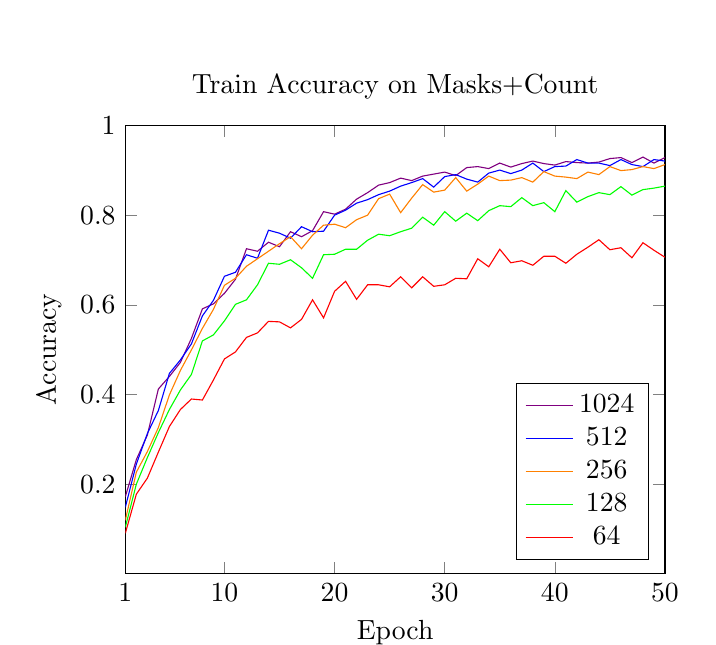
\begin{tikzpicture}
        \begin{axis}[
            title={Train Accuracy on Masks+Count},
            xlabel={Epoch},
            ylabel={Accuracy},
            xmin=1, xmax=50,
            ymin=0, ymax=1,
            xtick={1,10,20,30,40,50},
            ytick={0.2,0.4,0.6,0.8,1.0},
            legend pos=south east,
            %ymajorgrids=true,
            %grid style=dashed,
        ]

        \addplot[color=violet]
            coordinates{
                (1, 0.1720670461654663) (2, 0.2547486126422882) (3, 0.309497207403183) (4, 0.4122905135154724) (5, 0.44022345542907715) (6, 0.4715083837509155) (7, 0.5251396894454956) (8, 0.5910614728927612) (9, 0.6022346615791321) (10, 0.6256983280181885) (11, 0.6569832563400269) (12, 0.7251396775245667) (13, 0.7195530533790588) (14, 0.7396647930145264) (15, 0.729608952999115) (16, 0.7631285190582275) (17, 0.7519553303718567) (18, 0.7653631567955017) (19, 0.8078212141990662) (20, 0.8022346496582031) (21, 0.813407838344574) (22, 0.8357542157173157) (23, 0.8502793312072754) (24, 0.8670390844345093) (25, 0.8726257085800171) (26, 0.8826815485954285) (27, 0.8770949840545654) (28, 0.8871508240699768) (29, 0.8916200995445251) (30, 0.8960893750190735) (31, 0.8882681727409363) (32, 0.9061452746391296) (33, 0.9083799123764038) (34, 0.9039106369018555) (35, 0.916201114654541) (36, 0.9072625637054443) (37, 0.9150838255882263) (38, 0.9206703901290894) (39, 0.9150838255882263) (40, 0.9117318391799927) (41, 0.9195531010627747) (42, 0.9173184633255005) (43, 0.916201114654541) (44, 0.9184357523918152) (45, 0.9262569546699524) (46, 0.9284915924072266) (47, 0.9173184633255005) (48, 0.929608941078186) (49, 0.916201114654541) (50, 0.9284915924072266)
            };
            \addlegendentry{1024}

        \addplot[color=blue]
            coordinates{
                (1, 0.14860334992408752) (2, 0.24469274282455444) (3, 0.31284916400909424) (4, 0.36424580216407776) (5, 0.44692736864089966) (6, 0.47709497809410095) (7, 0.5128491520881653) (8, 0.575419008731842) (9, 0.6100558638572693) (10, 0.6636871695518494) (11, 0.672625720500946) (12, 0.7117318511009216) (13, 0.7039105892181396) (14, 0.7664804458618164) (15, 0.7597765326499939) (16, 0.748603343963623) (17, 0.7743016481399536) (18, 0.7631285190582275) (19, 0.7642458081245422) (20, 0.800000011920929) (21, 0.8111732006072998) (22, 0.826815664768219) (23, 0.8346368670463562) (24, 0.845810055732727) (25, 0.8536312580108643) (26, 0.8648044466972351) (27, 0.8726257085800171) (28, 0.8815642595291138) (29, 0.8625698089599609) (30, 0.8860335350036621) (31, 0.8905028104782104) (32, 0.8804469108581543) (33, 0.8737429976463318) (34, 0.8938547372817993) (35, 0.9005586504936218) (36, 0.8927374482154846) (37, 0.9005586504936218) (38, 0.916201114654541) (39, 0.897206723690033) (40, 0.9083799123764038) (41, 0.9094972014427185) (42, 0.9240223169326782) (43, 0.916201114654541) (44, 0.916201114654541) (45, 0.910614550113678) (46, 0.9240223169326782) (47, 0.9128491878509521) (48, 0.9083799123764038) (49, 0.9240223169326782) (50, 0.9206703901290894) 
            };
            \addlegendentry{512}

        \addplot[color=orange]
            coordinates{
                (1, 0.11955307424068451) (2, 0.22681564092636108) (3, 0.2726256847381592) (4, 0.32625699043273926) (5, 0.3988826870918274) (6, 0.45363128185272217) (7, 0.49944132566452026) (8, 0.5474860072135925) (9, 0.5899441242218018) (10, 0.6435754299163818) (11, 0.659217894077301) (12, 0.6860335469245911) (13, 0.702793300151825) (14, 0.7195530533790588) (15, 0.7363128662109375) (16, 0.7519553303718567) (17, 0.7251396775245667) (18, 0.7553072571754456) (19, 0.7776536345481873) (20, 0.7798882722854614) (21, 0.7720670104026794) (22, 0.7899441123008728) (23, 0.800000011920929) (24, 0.8368715047836304) (25, 0.8469273447990417) (26, 0.805586576461792) (27, 0.8379888534545898) (28, 0.8681564331054688) (29, 0.8513966202735901) (30, 0.8558658957481384) (31, 0.8837988972663879) (32, 0.8536312580108643) (33, 0.8692737221717834) (34, 0.8871508240699768) (35, 0.8770949840545654) (36, 0.8782122731208801) (37, 0.8837988972663879) (38, 0.8737429976463318) (39, 0.897206723690033) (40, 0.8871508240699768) (41, 0.8849161863327026) (42, 0.8815642595291138) (43, 0.8960893750190735) (44, 0.8905028104782104) (45, 0.9083799123764038) (46, 0.8994413614273071) (47, 0.9016759991645813) (48, 0.9083799123764038) (49, 0.9039106369018555) (50, 0.9128491878509521)
            };
            \addlegendentry{256}

        \addplot[color=green]
            coordinates{
                (1, 0.10391061753034592) (2, 0.20000000298023224) (3, 0.25921788811683655) (4, 0.3150838017463684) (5, 0.36648043990135193) (6, 0.41005587577819824) (7, 0.4446927309036255) (8, 0.5195530652999878) (9, 0.5329608917236328) (10, 0.5642458200454712) (11, 0.6011173129081726) (12, 0.6111732125282288) (13, 0.6446927189826965) (14, 0.6927374601364136) (15, 0.6905027627944946) (16, 0.7005586624145508) (17, 0.6826815605163574) (18, 0.659217894077301) (19, 0.7117318511009216) (20, 0.7128491401672363) (21, 0.7240223288536072) (22, 0.7240223288536072) (23, 0.7441340684890747) (24, 0.7575418949127197) (25, 0.7541899681091309) (26, 0.7631285190582275) (27, 0.7709497213363647) (28, 0.7955307364463806) (29, 0.7776536345481873) (30, 0.8078212141990662) (31, 0.7865921854972839) (32, 0.8044692873954773) (33, 0.7877094745635986) (34, 0.8100558519363403) (35, 0.8212290406227112) (36, 0.818994402885437) (37, 0.8391061425209045) (38, 0.8212290406227112) (39, 0.8279329538345337) (40, 0.8078212141990662) (41, 0.8547486066818237) (42, 0.8290503025054932) (43, 0.8413407802581787) (44, 0.8502793312072754) (45, 0.845810055732727) (46, 0.8636871576309204) (47, 0.8446927070617676) (48, 0.8569832444190979) (49, 0.8603351712226868) (50, 0.8648044466972351)
            };
            \addlegendentry{128}

        \addplot[color=red]
            coordinates{
                (1, 0.0905027911067009) (2, 0.17765362560749054) (3, 0.21340781450271606) (4, 0.2715083658695221) (5, 0.3284916281700134) (6, 0.36648043990135193) (7, 0.3899441361427307) (8, 0.38770949840545654) (9, 0.43240222334861755) (10, 0.4793296158313751) (11, 0.4949720799922943) (12, 0.5273743271827698) (13, 0.5374301671981812) (14, 0.5631284713745117) (15, 0.562011182308197) (16, 0.548603355884552) (17, 0.5675977468490601) (18, 0.6111732125282288) (19, 0.5709497332572937) (20, 0.6301676034927368) (21, 0.6525139808654785) (22, 0.6122905015945435) (23, 0.6446927189826965) (24, 0.6446927189826965) (25, 0.6402234435081482) (26, 0.6625698208808899) (27, 0.637988805770874) (28, 0.6625698208808899) (29, 0.6413407921791077) (30, 0.6446927189826965) (31, 0.659217894077301) (32, 0.6581005454063416) (33, 0.702793300151825) (34, 0.6849161982536316) (35, 0.7240223288536072) (36, 0.6938547492027283) (37, 0.6983240246772766) (38, 0.6882681846618652) (39, 0.708379864692688) (40, 0.708379864692688) (41, 0.6927374601364136) (42, 0.7128491401672363) (43, 0.7284916043281555) (44, 0.7452514171600342) (45, 0.7229050397872925) (46, 0.7273743152618408) (47, 0.7050279378890991) (48, 0.7385475039482117) (49, 0.721787691116333) (50, 0.7061452269554138)
            };
            \addlegendentry{64}

        \end{axis}
    \end{tikzpicture}
    \caption{The plot shows the how the train accuracy
        varies for the dataset Masks+Count changing the number
        of hidden nodes in the LSTM.}
    \label{fig:train-accuracy-masks+count}
\end{figure}

\begin{figure}
    \centering
    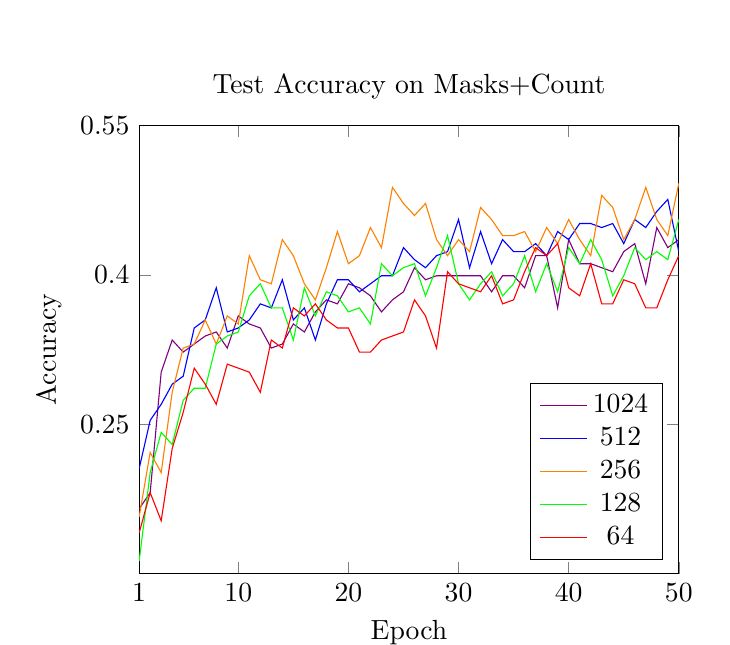
\begin{tikzpicture}
        \begin{axis}[
            title={Test Accuracy on Masks+Count},
            xlabel={Epoch},
            ylabel={Accuracy},
            xmin=1, xmax=50,
            ymin=0.1, ymax=0.55,
            xtick={1,10,20,30,40,50},
            ytick={0.25,0.40,0.55},
            legend pos=south east,
            %ymajorgrids=true,
            %grid style=dashed,
        ]

        \addplot[color=violet]
            coordinates{
                (1, 0.16532258689403534) (2, 0.18145161867141724) (3, 0.30241936445236206) (4, 0.33467742800712585) (5, 0.32258063554763794) (6, 0.3306451737880707) (7, 0.33870968222618103) (8, 0.3427419364452362) (9, 0.3266128897666931) (10, 0.3588709831237793) (11, 0.35080644488334656) (12, 0.3467741906642914) (13, 0.3266128897666931) (14, 0.3306451737880707) (15, 0.35080644488334656) (16, 0.3427419364452362) (17, 0.3629032373428345) (18, 0.375) (19, 0.3709677457809448) (20, 0.3911290466785431) (21, 0.3870967626571655) (22, 0.3790322542190552) (23, 0.3629032373428345) (24, 0.375) (25, 0.38306450843811035) (26, 0.4072580635547638) (27, 0.39516130089759827) (28, 0.39919355511665344) (29, 0.39919355511665344) (30, 0.39919355511665344) (31, 0.39919355511665344) (32, 0.39919355511665344) (33, 0.38306450843811035) (34, 0.39919355511665344) (35, 0.39919355511665344) (36, 0.3870967626571655) (37, 0.4193548262119293) (38, 0.4193548262119293) (39, 0.36693549156188965) (40, 0.4354838728904724) (41, 0.41129031777381897) (42, 0.41129031777381897) (43, 0.4072580635547638) (44, 0.4032258093357086) (45, 0.4233870804309845) (46, 0.43145161867141724) (47, 0.3911290168762207) (48, 0.44758063554763794) (49, 0.42741936445236206) (50, 0.4354838728904724) 
            };
            \addlegendentry{1024}

        \addplot[color=blue]
            coordinates{
                (1, 0.20564515888690948) (2, 0.2540322542190552) (3, 0.27016130089759827) (4, 0.29032257199287415) (5, 0.2983871102333069) (6, 0.3467741906642914) (7, 0.35483869910240173) (8, 0.3870967626571655) (9, 0.3427419364452362) (10, 0.3467741906642914) (11, 0.35483869910240173) (12, 0.3709677457809448) (13, 0.36693549156188965) (14, 0.39516130089759827) (15, 0.35483869910240173) (16, 0.36693549156188965) (17, 0.33467742800712585) (18, 0.3709677457809448) (19, 0.39516130089759827) (20, 0.39516130089759827) (21, 0.38306450843811035) (22, 0.3911290466785431) (23, 0.39919355511665344) (24, 0.39919355511665344) (25, 0.42741936445236206) (26, 0.41532257199287415) (27, 0.4072580635547638) (28, 0.4193548262119293) (29, 0.4233871102333069) (30, 0.4556451737880707) (31, 0.4072580635547638) (32, 0.44354838132858276) (33, 0.41129031777381897) (34, 0.4354838728904724) (35, 0.4233871102333069) (36, 0.4233871102333069) (37, 0.43145161867141724) (38, 0.4193548262119293) (39, 0.44354838132858276) (40, 0.4354838728904724) (41, 0.4516128897666931) (42, 0.4516129195690155) (43, 0.44758063554763794) (44, 0.4516129195690155) (45, 0.43145161867141724) (46, 0.4556451737880707) (47, 0.44758063554763794) (48, 0.46370968222618103) (49, 0.47580644488334656) (50, 0.4233871102333069)
            };
            \addlegendentry{512}

        \addplot[color=orange]
            coordinates{
                (1, 0.1572580635547638) (2, 0.22177419066429138) (3, 0.2016129046678543) (4, 0.2822580635547638) (5, 0.3266129195690155) (6, 0.3306451737880707) (7, 0.35483869910240173) (8, 0.3306451737880707) (9, 0.3588709533214569) (10, 0.35080644488334656) (11, 0.4193548262119293) (12, 0.39516130089759827) (13, 0.3911290466785431) (14, 0.4354838728904724) (15, 0.4193548262119293) (16, 0.3911290466785431) (17, 0.375) (18, 0.4072580635547638) (19, 0.44354838132858276) (20, 0.41129031777381897) (21, 0.4193548262119293) (22, 0.44758063554763794) (23, 0.42741936445236206) (24, 0.4879032373428345) (25, 0.4717741906642914) (26, 0.45967742800712585) (27, 0.4717741906642914) (28, 0.4354838728904724) (29, 0.4193548262119293) (30, 0.4354838728904724) (31, 0.4233871102333069) (32, 0.4677419364452362) (33, 0.4556451737880707) (34, 0.4395161271095276) (35, 0.4395161271095276) (36, 0.44354838132858276) (37, 0.4233871102333069) (38, 0.44758063554763794) (39, 0.43145161867141724) (40, 0.4556451737880707) (41, 0.4354838728904724) (42, 0.4193548262119293) (43, 0.47983869910240173) (44, 0.4677419364452362) (45, 0.4354838728904724) (46, 0.4556451737880707) (47, 0.4879032373428345) (48, 0.4556451737880707) (49, 0.4395161271095276) (50, 0.49193549156188965)
            };
            \addlegendentry{256}

        \addplot[color=green]
            coordinates{
                (1, 0.11290322244167328) (2, 0.2016129046678543) (3, 0.24193547666072845) (4, 0.22983871400356293) (5, 0.27419355511665344) (6, 0.28629031777381897) (7, 0.28629031777381897) (8, 0.3306451737880707) (9, 0.33870968222618103) (10, 0.3427419364452362) (11, 0.3790322542190552) (12, 0.3911290466785431) (13, 0.36693549156188965) (14, 0.36693549156188965) (15, 0.33467742800712585) (16, 0.3870967626571655) (17, 0.3588709831237793) (18, 0.38306450843811035) (19, 0.3790322542190552) (20, 0.3629032373428345) (21, 0.36693549156188965) (22, 0.35080644488334656) (23, 0.41129031777381897) (24, 0.39919355511665344) (25, 0.4072580635547638) (26, 0.41129031777381897) (27, 0.3790322542190552) (28, 0.4072580635547638) (29, 0.4395161271095276) (30, 0.3911290466785431) (31, 0.375) (32, 0.3911290466785431) (33, 0.4032258093357086) (34, 0.3790322542190552) (35, 0.3911290466785431) (36, 0.4193548262119293) (37, 0.38306450843811035) (38, 0.41129031777381897) (39, 0.38306450843811035) (40, 0.42741936445236206) (41, 0.41129031777381897) (42, 0.4354838728904724) (43, 0.41532257199287415) (44, 0.3790322542190552) (45, 0.39919355511665344) (46, 0.42741936445236206) (47, 0.41532257199287415) (48, 0.4233870804309845) (49, 0.41532257199287415) (50, 0.4556451737880707) 
            };
            \addlegendentry{128}

        \addplot[color=red]
            coordinates{
                (1, 0.1411290317773819) (2, 0.18145161867141724) (3, 0.15322580933570862) (4, 0.22580644488334656) (5, 0.2620967626571655) (6, 0.30645161867141724) (7, 0.29032257199287415) (8, 0.27016130089759827) (9, 0.3104838728904724) (10, 0.30645161867141724) (11, 0.30241936445236206) (12, 0.2822580635547638) (13, 0.33467742800712585) (14, 0.3266128897666931) (15, 0.36693549156188965) (16, 0.3588709533214569) (17, 0.3709677457809448) (18, 0.35483869910240173) (19, 0.3467741906642914) (20, 0.3467741906642914) (21, 0.32258063554763794) (22, 0.32258063554763794) (23, 0.33467742800712585) (24, 0.33870968222618103) (25, 0.3427419364452362) (26, 0.375) (27, 0.3588709831237793) (28, 0.3266128897666931) (29, 0.4032258093357086) (30, 0.3911290466785431) (31, 0.3870967626571655) (32, 0.38306450843811035) (33, 0.39919355511665344) (34, 0.3709677457809448) (35, 0.375) (36, 0.4032258093357086) (37, 0.42741936445236206) (38, 0.4193548262119293) (39, 0.43145161867141724) (40, 0.3870967626571655) (41, 0.3790322542190552) (42, 0.41129031777381897) (43, 0.3709677457809448) (44, 0.3709677457809448) (45, 0.39516130089759827) (46, 0.3911290466785431) (47, 0.36693549156188965) (48, 0.36693549156188965) (49, 0.39516130089759827) (50, 0.4193548262119293) 
            };
            \addlegendentry{64}

        \end{axis}
    \end{tikzpicture}
    \caption{The plot shows the how the test accuracy
        varies for the dataset Masks+Count changing the number
        of hidden nodes in the LSTM.}
    \label{fig:test-accuracy-masks+count}
\end{figure}

\begin{figure}
    \centering
    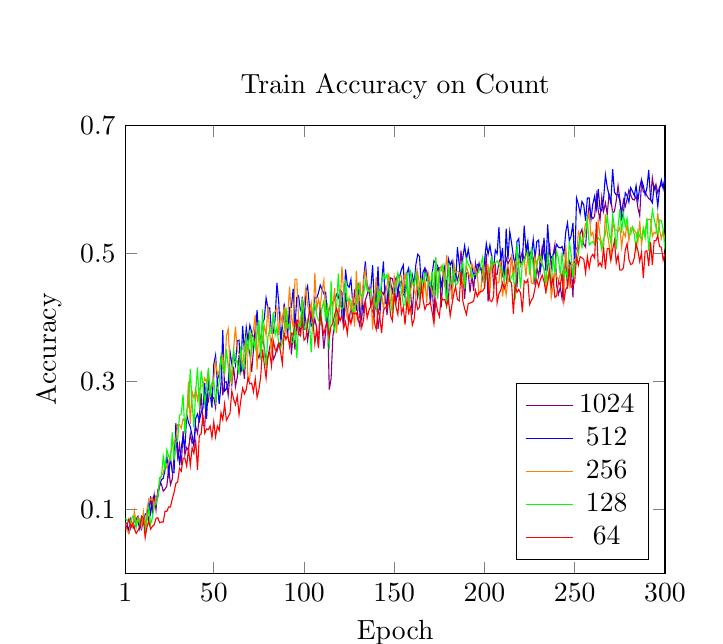
\begin{tikzpicture}
        \begin{axis}[
            title={Train Accuracy on Count},
            xlabel={Epoch},
            ylabel={Accuracy},
            xmin=1, xmax=300,
            ymin=0, ymax=0.7,
            xtick={1,50,100,150,200,250,300},
            ytick={0.1,0.3,0.5,0.7},
            legend pos=south east,
            %ymajorgrids=true,
            %grid style=dashed,
        ]

        \addplot[color=violet]
            coordinates{
                (1, 0.07039105892181396) (2, 0.07374301552772522) (3, 0.06368715316057205) (4, 0.07150837779045105) (5, 0.0748603343963623) (6, 0.06927374005317688) (7, 0.08491620421409607) (8, 0.08938547223806381) (9, 0.07597765326499939) (10, 0.06927374005317688) (11, 0.08491620421409607) (12, 0.07374301552772522) (13, 0.09273742884397507) (14, 0.08156424760818481) (15, 0.1206703931093216) (16, 0.09720670431852341) (17, 0.12290503084659576) (18, 0.09944134205579758) (19, 0.13072626292705536) (20, 0.13743016123771667) (21, 0.13966479897499084) (22, 0.1284916251897812) (23, 0.13184358179569244) (24, 0.1363128423690796) (25, 0.1653631329536438) (26, 0.13854748010635376) (27, 0.14748603105545044) (28, 0.18435753881931305) (29, 0.21340781450271606) (30, 0.1810055822134018) (31, 0.20111732184886932) (32, 0.16871508955955505) (33, 0.22234636545181274) (34, 0.18547485768795013) (35, 0.19664804637432098) (36, 0.19217877089977264) (37, 0.2178770899772644) (38, 0.2033519595861435) (39, 0.20670391619205475) (40, 0.22905027866363525) (41, 0.2189944088459015) (42, 0.24469274282455444) (43, 0.28156423568725586) (44, 0.23128491640090942) (45, 0.23016759753227234) (46, 0.2782122790813446) (47, 0.2692737281322479) (48, 0.28938546776771545) (49, 0.2726256847381592) (50, 0.27486032247543335) (51, 0.25921788811683655) (52, 0.3016759753227234) (53, 0.31173184514045715) (54, 0.3396648168563843) (55, 0.2782122790813446) (56, 0.29832401871681213) (57, 0.2994413375854492) (58, 0.2782122790813446) (59, 0.31173184514045715) (60, 0.2949720621109009) (61, 0.322905033826828) (62, 0.2916201055049896) (63, 0.30614525079727173) (64, 0.34078213572502136) (65, 0.3139664828777313) (66, 0.32737430930137634) (67, 0.30391061305999756) (68, 0.35865920782089233) (69, 0.35642457008361816) (70, 0.34301677346229553) (71, 0.3150838017463684) (72, 0.34860333800315857) (73, 0.3854748606681824) (74, 0.3441340923309326) (75, 0.336312860250473) (76, 0.34860333800315857) (77, 0.367597758769989) (78, 0.3530726134777069) (79, 0.32737430930137634) (80, 0.3374301791191101) (81, 0.3530726134777069) (82, 0.36424580216407776) (83, 0.33407822251319885) (84, 0.34078213572502136) (85, 0.3519552946090698) (86, 0.3608938455581665) (87, 0.3553072512149811) (88, 0.3843575417995453) (89, 0.4212290644645691) (90, 0.39441341161727905) (91, 0.3921787738800049) (92, 0.4078212380409241) (93, 0.34189945459365845) (94, 0.3754189908504486) (95, 0.34972065687179565) (96, 0.39329609274864197) (97, 0.3966480493545532) (98, 0.3698323965072632) (99, 0.43240222334861755) (100, 0.4111731946468353) (101, 0.39441341161727905) (102, 0.36424580216407776) (103, 0.3854748606681824) (104, 0.40893855690956116) (105, 0.3832402229309082) (106, 0.3977653682231903) (107, 0.3832402229309082) (108, 0.3553072512149811) (109, 0.42458099126815796) (110, 0.3854748606681824) (111, 0.35083797574043274) (112, 0.3776536285877228) (113, 0.4122905135154724) (114, 0.2871508300304413) (115, 0.30391061305999756) (116, 0.37094971537590027) (117, 0.38770949840545654) (118, 0.4134078323841095) (119, 0.38882681727409363) (120, 0.4435754120349884) (121, 0.40223464369773865) (122, 0.3921787738800049) (123, 0.437988817691803) (124, 0.4078212380409241) (125, 0.39553073048591614) (126, 0.41564247012138367) (127, 0.4000000059604645) (128, 0.4435754120349884) (129, 0.4223463833332062) (130, 0.3988826870918274) (131, 0.3854748606681824) (132, 0.4346368610858917) (133, 0.41005587577819824) (134, 0.42681562900543213) (135, 0.4357541799545288) (136, 0.44692736864089966) (137, 0.41675978899002075) (138, 0.40893855690956116) (139, 0.40223464369773865) (140, 0.44804468750953674) (141, 0.3821229040622711) (142, 0.40223464369773865) (143, 0.44022345542907715) (144, 0.4357541799545288) (145, 0.4458100497722626) (146, 0.40335196256637573) (147, 0.4446927309036255) (148, 0.46145251393318176) (149, 0.4603351950645447) (150, 0.4446927309036255) (151, 0.42458099126815796) (152, 0.4435754120349884) (153, 0.4525139629840851) (154, 0.4569832384586334) (155, 0.4357541799545288) (156, 0.4446927309036255) (157, 0.44692736864089966) (158, 0.4279329478740692) (159, 0.44022345542907715) (160, 0.4044692814350128) (161, 0.45363128185272217) (162, 0.47039106488227844) (163, 0.43128490447998047) (164, 0.4458100497722626) (165, 0.4458100497722626) (166, 0.4435754120349884) (167, 0.47597765922546387) (168, 0.4726257026195526) (169, 0.4569832384586334) (170, 0.4223463535308838) (171, 0.4502793252468109) (172, 0.3988826870918274) (173, 0.46368715167045593) (174, 0.47597765922546387) (175, 0.47709497809410095) (176, 0.41564247012138367) (177, 0.4603351950645447) (178, 0.45586591958999634) (179, 0.437988817691803) (180, 0.42569831013679504) (181, 0.47821229696273804) (182, 0.4279329478740692) (183, 0.4815642535686493) (184, 0.4670391082763672) (185, 0.4581005573272705) (186, 0.46927374601364136) (187, 0.5039106011390686) (188, 0.4681564271450043) (189, 0.4290502667427063) (190, 0.46927374601364136) (191, 0.46927374601364136) (192, 0.43910613656044006) (193, 0.4659217894077301) (194, 0.44134077429771423) (195, 0.48491621017456055) (196, 0.4681564271450043) (197, 0.48491621017456055) (198, 0.4737430214881897) (199, 0.4726257026195526) (200, 0.4569832384586334) (201, 0.49944135546684265) (202, 0.42458099126815796) (203, 0.4715083837509155) (204, 0.4972067177295685) (205, 0.451396644115448) (206, 0.4670391082763672) (207, 0.4670391082763672) (208, 0.48603352904319763) (209, 0.49273744225502014) (210, 0.464804470539093) (211, 0.47039106488227844) (212, 0.49273744225502014) (213, 0.48379889130592346) (214, 0.4893854856491089) (215, 0.4949720799922943) (216, 0.4670391082763672) (217, 0.49162012338638306) (218, 0.44692736864089966) (219, 0.4972067177295685) (220, 0.49162012338638306) (221, 0.5027933120727539) (222, 0.4893854856491089) (223, 0.49944132566452026) (224, 0.5117318630218506) (225, 0.4972067177295685) (226, 0.5039106011390686) (227, 0.49273744225502014) (228, 0.4502793252468109) (229, 0.47821229696273804) (230, 0.46368715167045593) (231, 0.4871508479118347) (232, 0.5106145143508911) (233, 0.49832403659820557) (234, 0.48379889130592346) (235, 0.4748603403568268) (236, 0.5162011384963989) (237, 0.47709497809410095) (238, 0.4972067177295685) (239, 0.5139665007591248) (240, 0.44916200637817383) (241, 0.4357541799545288) (242, 0.44692736864089966) (243, 0.4290502667427063) (244, 0.46927374601364136) (245, 0.49050280451774597) (246, 0.4446927309036255) (247, 0.4882681667804718) (248, 0.4815642535686493) (249, 0.43128490447998047) (250, 0.5117318630218506) (251, 0.5072625875473022) (252, 0.5027933120727539) (253, 0.5307262539863586) (254, 0.5374301671981812) (255, 0.5139665007591248) (256, 0.5094972252845764) (257, 0.5519552826881409) (258, 0.575419008731842) (259, 0.5597765445709229) (260, 0.554189920425415) (261, 0.5575419068336487) (262, 0.5910614728927612) (263, 0.5675977468490601) (264, 0.5519552826881409) (265, 0.5877094864845276) (266, 0.5653631091117859) (267, 0.5787709355354309) (268, 0.5608938336372375) (269, 0.5921787619590759) (270, 0.5843575596809387) (271, 0.5631284713745117) (272, 0.5653631091117859) (273, 0.5821229219436646) (274, 0.605586588382721) (275, 0.5843575596809387) (276, 0.562011182308197) (277, 0.5832402110099792) (278, 0.5731843709945679) (279, 0.5843575596809387) (280, 0.5988826751708984) (281, 0.5910614728927612) (282, 0.5843575596809387) (283, 0.5832402110099792) (284, 0.5899441242218018) (285, 0.5709497332572937) (286, 0.5586591958999634) (287, 0.6122905015945435) (288, 0.5955307483673096) (289, 0.5955307483673096) (290, 0.5899441242218018) (291, 0.5854748487472534) (292, 0.5832402110099792) (293, 0.6178770661354065) (294, 0.5988826751708984) (295, 0.6078212261199951) (296, 0.5944133996963501) (297, 0.6033519506454468) (298, 0.6067039370536804) (299, 0.6033519506454468) (300, 0.6156424880027771) 
            };
            \addlegendentry{1024}

        \addplot[color=blue]
            coordinates{(1, 0.07932960987091064) (2, 0.07821229100227356) (3, 0.06592179089784622) (4, 0.08491620421409607) (5, 0.07597765326499939) (6, 0.08156424760818481) (7, 0.08491620421409607) (8, 0.08156424760818481) (9, 0.06927374005317688) (10, 0.08603352308273315) (11, 0.07821229100227356) (12, 0.09273742884397507) (13, 0.09385474771261215) (14, 0.11173184216022491) (15, 0.09385474771261215) (16, 0.112849161028862) (17, 0.12178771197795868) (18, 0.11955307424068451) (19, 0.11955307424068451) (20, 0.13743016123771667) (21, 0.14636871218681335) (22, 0.14860334992408752) (23, 0.16201117634773254) (24, 0.18324021995067596) (25, 0.15530726313591003) (26, 0.1810055822134018) (27, 0.1586592197418213) (28, 0.1575419008731842) (29, 0.23463687300682068) (30, 0.19441340863704681) (31, 0.1731843501329422) (32, 0.19664804637432098) (33, 0.21340781450271606) (34, 0.19441340863704681) (35, 0.2491620033979416) (36, 0.23575419187545776) (37, 0.22905027866363525) (38, 0.21564245223999023) (39, 0.19888268411159515) (40, 0.24245810508728027) (41, 0.2491620033979416) (42, 0.23798882961273193) (43, 0.25139665603637695) (44, 0.25810056924819946) (45, 0.29720669984817505) (46, 0.2413407862186432) (47, 0.29832401871681213) (48, 0.2804469168186188) (49, 0.25921788811683655) (50, 0.32625699043273926) (51, 0.34078213572502136) (52, 0.29720669984817505) (53, 0.264804482460022) (54, 0.2938547432422638) (55, 0.37988826632499695) (56, 0.2849161922931671) (57, 0.28826814889907837) (58, 0.29720669984817505) (59, 0.3463687002658844) (60, 0.32737430930137634) (61, 0.34301677346229553) (62, 0.32625699043273926) (63, 0.3631284832954407) (64, 0.36424580216407776) (65, 0.3150838017463684) (66, 0.38659217953681946) (67, 0.3463687002658844) (68, 0.3843575417995453) (69, 0.3631284832954407) (70, 0.38770949840545654) (71, 0.3765363097190857) (72, 0.367597758769989) (73, 0.3743016719818115) (74, 0.4111731946468353) (75, 0.36536312103271484) (76, 0.36648043990135193) (77, 0.3899441361427307) (78, 0.3977653682231903) (79, 0.4301675856113434) (80, 0.4145251512527466) (81, 0.4145251512527466) (82, 0.3754189908504486) (83, 0.3754189908504486) (84, 0.3977653682231903) (85, 0.45363128185272217) (86, 0.4234636723995209) (87, 0.36536312103271484) (88, 0.38882681727409363) (89, 0.41564247012138367) (90, 0.38882681727409363) (91, 0.3754189908504486) (92, 0.41564247012138367) (93, 0.41564247012138367) (94, 0.4446927309036255) (95, 0.3843575417995453) (96, 0.43128490447998047) (97, 0.43351954221725464) (98, 0.4111731946468353) (99, 0.41675978899002075) (100, 0.37988826632499695) (101, 0.44022345542907715) (102, 0.44916200637817383) (103, 0.41675978899002075) (104, 0.38659217953681946) (105, 0.3899441361427307) (106, 0.43128490447998047) (107, 0.4301675856113434) (108, 0.437988817691803) (109, 0.4502793252468109) (110, 0.4435754120349884) (111, 0.4368714988231659) (112, 0.43910613656044006) (113, 0.3966480493545532) (114, 0.4145251512527466) (115, 0.420111745595932) (116, 0.4234636723995209) (117, 0.4279329478740692) (118, 0.4357541799545288) (119, 0.4301675856113434) (120, 0.4424580931663513) (121, 0.43910613656044006) (122, 0.3899441361427307) (123, 0.4748603403568268) (124, 0.4502793252468109) (125, 0.44692736864089966) (126, 0.4592178761959076) (127, 0.4223463535308838) (128, 0.4212290644645691) (129, 0.4134078323841095) (130, 0.45363128185272217) (131, 0.4044692814350128) (132, 0.3966480493545532) (133, 0.4592178761959076) (134, 0.4871508479118347) (135, 0.44804468750953674) (136, 0.43910613656044006) (137, 0.4435754120349884) (138, 0.4815642535686493) (139, 0.41675978899002075) (140, 0.4134078323841095) (141, 0.4793296158313751) (142, 0.4111731946468353) (143, 0.45363128185272217) (144, 0.4871508479118347) (145, 0.4223463535308838) (146, 0.4223463833332062) (147, 0.45586591958999634) (148, 0.45363128185272217) (149, 0.43910613656044006) (150, 0.45474860072135925) (151, 0.46145251393318176) (152, 0.43128490447998047) (153, 0.46368715167045593) (154, 0.4748603403568268) (155, 0.4815642535686493) (156, 0.4301675856113434) (157, 0.46927374601364136) (158, 0.47709497809410095) (159, 0.4435754120349884) (160, 0.4659217894077301) (161, 0.4525139629840851) (162, 0.4826815724372864) (163, 0.49832403659820557) (164, 0.4949720799922943) (165, 0.44804468750953674) (166, 0.4715083837509155) (167, 0.47709497809410095) (168, 0.4581005573272705) (169, 0.46256983280181885) (170, 0.4290502667427063) (171, 0.4681564271450043) (172, 0.4882681667804718) (173, 0.48491621017456055) (174, 0.4804469347000122) (175, 0.47039106488227844) (176, 0.44804468750953674) (177, 0.464804470539093) (178, 0.4793296158313751) (179, 0.4368714988231659) (180, 0.49162012338638306) (181, 0.4815642535686493) (182, 0.4882681667804718) (183, 0.4603351950645447) (184, 0.45363128185272217) (185, 0.5094972252845764) (186, 0.4826815724372864) (187, 0.46145251393318176) (188, 0.4938547611236572) (189, 0.5117318630218506) (190, 0.49050280451774597) (191, 0.5061452388763428) (192, 0.4882681667804718) (193, 0.4793296158313751) (194, 0.4659217894077301) (195, 0.46145251393318176) (196, 0.4826815724372864) (197, 0.4815642535686493) (198, 0.47821229696273804) (199, 0.4603351950645447) (200, 0.4871508479118347) (201, 0.5150837898254395) (202, 0.49832403659820557) (203, 0.5128491520881653) (204, 0.4938547611236572) (205, 0.4748603403568268) (206, 0.5050279498100281) (207, 0.49944132566452026) (208, 0.54078209400177) (209, 0.4882681667804718) (210, 0.5083798766136169) (211, 0.45363128185272217) (212, 0.5385474562644958) (213, 0.49050280451774597) (214, 0.5340782403945923) (215, 0.5162011384963989) (216, 0.4949720799922943) (217, 0.4815642535686493) (218, 0.5184357762336731) (219, 0.5229050517082214) (220, 0.4815642535686493) (221, 0.4882681667804718) (222, 0.5430167317390442) (223, 0.5039106011390686) (224, 0.5184357762336731) (225, 0.47709497809410095) (226, 0.4960893988609314) (227, 0.521787703037262) (228, 0.49162012338638306) (229, 0.5184357762336731) (230, 0.5206704139709473) (231, 0.4737430214881897) (232, 0.49273744225502014) (233, 0.5240223407745361) (234, 0.4726257026195526) (235, 0.5452513694763184) (236, 0.5005586743354797) (237, 0.49273744225502014) (238, 0.4972067177295685) (239, 0.5027933120727539) (240, 0.5139665007591248) (241, 0.5094972252845764) (242, 0.5083798766136169) (243, 0.5106145143508911) (244, 0.49832403659820557) (245, 0.5329608917236328) (246, 0.5474860072135925) (247, 0.5195530652999878) (248, 0.5273743271827698) (249, 0.5474860072135925) (250, 0.4804469347000122) (251, 0.5865921974182129) (252, 0.5765362977981567) (253, 0.562011182308197) (254, 0.5810055732727051) (255, 0.575419008731842) (256, 0.5508379936218262) (257, 0.5865921974182129) (258, 0.5865921974182129) (259, 0.5530726313591003) (260, 0.5765362977981567) (261, 0.5888268351554871) (262, 0.5698323845863342) (263, 0.6000000238418579) (264, 0.5698323845863342) (265, 0.5664804577827454) (266, 0.5854748487472534) (267, 0.6223463416099548) (268, 0.6033519506454468) (269, 0.5910614728927612) (270, 0.5787709355354309) (271, 0.6312848925590515) (272, 0.5955307483673096) (273, 0.5910614728927612) (274, 0.5921787619590759) (275, 0.5821229219436646) (276, 0.554189920425415) (277, 0.5631284713745117) (278, 0.5944133996963501) (279, 0.5899441242218018) (280, 0.5798882842063904) (281, 0.6022346615791321) (282, 0.5966480374336243) (283, 0.5899441242218018) (284, 0.605586588382721) (285, 0.5821229219436646) (286, 0.6033519506454468) (287, 0.6145251393318176) (288, 0.605586588382721) (289, 0.5910614728927612) (290, 0.6022346615791321) (291, 0.6301676034927368) (292, 0.5843575596809387) (293, 0.5787709355354309) (294, 0.6044692993164062) (295, 0.6000000238418579) (296, 0.5731843709945679) (297, 0.6011173129081726) (298, 0.6145251393318176) (299, 0.6011173129081726) (300, 0.618994414806366) };
            \addlegendentry{512}

        \addplot[color=orange]
            coordinates{
                (1, 0.07932960987091064) (2, 0.0670391097664833) (3, 0.06256983429193497) (4, 0.08156424760818481) (5, 0.07262569665908813) (6, 0.09720670431852341) (7, 0.07821229100227356) (8, 0.08715083450078964) (9, 0.08491620421409607) (10, 0.07262569665908813) (11, 0.09608938544988632) (12, 0.06927374005317688) (13, 0.09944134205579758) (14, 0.11620111763477325) (15, 0.11508379876613617) (16, 0.11843575537204742) (17, 0.10391061753034592) (18, 0.1206703931093216) (19, 0.12290503084659576) (20, 0.14525139331817627) (21, 0.15307262539863586) (22, 0.15642458200454712) (23, 0.17094972729682922) (24, 0.1653631329536438) (25, 0.17541898787021637) (26, 0.18547485768795013) (27, 0.20000000298023224) (28, 0.20558659732341766) (29, 0.210055872797966) (30, 0.2324022352695465) (31, 0.2324022352695465) (32, 0.22681564092636108) (33, 0.2413407862186432) (34, 0.23798882961273193) (35, 0.24469274282455444) (36, 0.2994413375854492) (37, 0.2335195541381836) (38, 0.28379887342453003) (39, 0.27374300360679626) (40, 0.28826814889907837) (41, 0.2703910768032074) (42, 0.28826814889907837) (43, 0.2927374243736267) (44, 0.2927374243736267) (45, 0.30502793192863464) (46, 0.29832401871681213) (47, 0.3162011206150055) (48, 0.28938546776771545) (49, 0.2927374243736267) (50, 0.30502793192863464) (51, 0.3307262659072876) (52, 0.31173184514045715) (53, 0.3150838017463684) (54, 0.3296089470386505) (55, 0.34078213572502136) (56, 0.3083798885345459) (57, 0.37094971537590027) (58, 0.3821229040622711) (59, 0.3217877149581909) (60, 0.29608938097953796) (61, 0.34972065687179565) (62, 0.3854748606681824) (63, 0.34972065687179565) (64, 0.34301677346229553) (65, 0.3374301791191101) (66, 0.322905033826828) (67, 0.3530726134777069) (68, 0.3698323965072632) (69, 0.3005586564540863) (70, 0.30502793192863464) (71, 0.37206703424453735) (72, 0.38100558519363403) (73, 0.40335196256637573) (74, 0.31843575835227966) (75, 0.38882681727409363) (76, 0.3452513813972473) (77, 0.36648043990135193) (78, 0.38659217953681946) (79, 0.37206703424453735) (80, 0.41787710785865784) (81, 0.3765363097190857) (82, 0.34189945459365845) (83, 0.4055866003036499) (84, 0.40893855690956116) (85, 0.4145251512527466) (86, 0.37206703424453735) (87, 0.4044692814350128) (88, 0.3899441361427307) (89, 0.41675978899002075) (90, 0.3743016719818115) (91, 0.40223464369773865) (92, 0.44804468750953674) (93, 0.4000000059604645) (94, 0.3843575417995453) (95, 0.4592178761959076) (96, 0.4592178761959076) (97, 0.3977653682231903) (98, 0.3843575417995453) (99, 0.38659217953681946) (100, 0.420111745595932) (101, 0.4458100497722626) (102, 0.41787710785865784) (103, 0.41005587577819824) (104, 0.4223463535308838) (105, 0.38659217953681946) (106, 0.46927374601364136) (107, 0.4122905135154724) (108, 0.4279329478740692) (109, 0.41564247012138367) (110, 0.4424580931663513) (111, 0.4581005573272705) (112, 0.4044692814350128) (113, 0.40223464369773865) (114, 0.41564247012138367) (115, 0.4223463535308838) (116, 0.41564247012138367) (117, 0.4458100497722626) (118, 0.3754189908504486) (119, 0.4122905135154724) (120, 0.41787710785865784) (121, 0.4793296158313751) (122, 0.43910613656044006) (123, 0.4122905135154724) (124, 0.3988826870918274) (125, 0.4301675856113434) (126, 0.4111731946468353) (127, 0.4290502667427063) (128, 0.3854748606681824) (129, 0.4726257026195526) (130, 0.41005587577819824) (131, 0.45586591958999634) (132, 0.4189944267272949) (133, 0.4569832384586334) (134, 0.4748603403568268) (135, 0.44692736864089966) (136, 0.44022345542907715) (137, 0.4435754120349884) (138, 0.38100558519363403) (139, 0.42458099126815796) (140, 0.46256983280181885) (141, 0.41675978899002075) (142, 0.44134077429771423) (143, 0.437988817691803) (144, 0.4134078323841095) (145, 0.43351954221725464) (146, 0.4502793252468109) (147, 0.4659217894077301) (148, 0.44916200637817383) (149, 0.4134078323841095) (150, 0.46368715167045593) (151, 0.44692736864089966) (152, 0.46145251393318176) (153, 0.46368715167045593) (154, 0.464804470539093) (155, 0.4368714988231659) (156, 0.4681564271450043) (157, 0.45474860072135925) (158, 0.40335196256637573) (159, 0.4424580931663513) (160, 0.4581005573272705) (161, 0.4424580931663513) (162, 0.43351954221725464) (163, 0.47039106488227844) (164, 0.44916200637817383) (165, 0.4603351950645447) (166, 0.43351954221725464) (167, 0.4592178761959076) (168, 0.4223463535308838) (169, 0.4670391082763672) (170, 0.4525139629840851) (171, 0.4357541799545288) (172, 0.4458100497722626) (173, 0.49273744225502014) (174, 0.43128490447998047) (175, 0.4726257026195526) (176, 0.4804469347000122) (177, 0.46927374601364136) (178, 0.44692736864089966) (179, 0.4972067177295685) (180, 0.46927374601364136) (181, 0.451396644115448) (182, 0.4290502667427063) (183, 0.48491621017456055) (184, 0.47039106488227844) (185, 0.4715083837509155) (186, 0.47039106488227844) (187, 0.464804470539093) (188, 0.44916200637817383) (189, 0.4659217894077301) (190, 0.4793296158313751) (191, 0.46927374601364136) (192, 0.46256983280181885) (193, 0.48379889130592346) (194, 0.4748603403568268) (195, 0.47597765922546387) (196, 0.4659217894077301) (197, 0.4357541799545288) (198, 0.44022345542907715) (199, 0.4815642535686493) (200, 0.4446927309036255) (201, 0.4793296158313751) (202, 0.4815642535686493) (203, 0.437988817691803) (204, 0.4882681667804718) (205, 0.4726257026195526) (206, 0.46256983280181885) (207, 0.45363128185272217) (208, 0.45474860072135925) (209, 0.4871508479118347) (210, 0.43240222334861755) (211, 0.45474860072135925) (212, 0.4346368610858917) (213, 0.4581005573272705) (214, 0.46145251393318176) (215, 0.49944132566452026) (216, 0.4581005573272705) (217, 0.4871508479118347) (218, 0.4815642535686493) (219, 0.4893854856491089) (220, 0.4815642535686493) (221, 0.48491621017456055) (222, 0.49050280451774597) (223, 0.46368715167045593) (224, 0.4960893988609314) (225, 0.4871508479118347) (226, 0.45363128185272217) (227, 0.4525139629840851) (228, 0.4938547611236572) (229, 0.4793296158313751) (230, 0.4972067177295685) (231, 0.48603352904319763) (232, 0.48379889130592346) (233, 0.4748603403568268) (234, 0.4368714988231659) (235, 0.46368715167045593) (236, 0.4748603403568268) (237, 0.43128490447998047) (238, 0.44804468750953674) (239, 0.46927374601364136) (240, 0.46368715167045593) (241, 0.4581005573272705) (242, 0.4659217894077301) (243, 0.4670391082763672) (244, 0.4357541799545288) (245, 0.5128491520881653) (246, 0.4681564271450043) (247, 0.4502793252468109) (248, 0.4804469347000122) (249, 0.4826815724372864) (250, 0.49050280451774597) (251, 0.49050280451774597) (252, 0.5340782403945923) (253, 0.5262569785118103) (254, 0.5139665007591248) (255, 0.5318436026573181) (256, 0.5463687181472778) (257, 0.5497206449508667) (258, 0.562011182308197) (259, 0.5273743271827698) (260, 0.5329608917236328) (261, 0.5139665007591248) (262, 0.5184357762336731) (263, 0.5508379936218262) (264, 0.5273743271827698) (265, 0.5150837898254395) (266, 0.5094972252845764) (267, 0.5608938336372375) (268, 0.5329608917236328) (269, 0.5139665007591248) (270, 0.49050280451774597) (271, 0.5474860072135925) (272, 0.5374301671981812) (273, 0.5363128781318665) (274, 0.5340782403945923) (275, 0.54078209400177) (276, 0.5094972252845764) (277, 0.5329608917236328) (278, 0.5262569785118103) (279, 0.5463687181472778) (280, 0.5195530652999878) (281, 0.5396648049354553) (282, 0.54078209400177) (283, 0.5363128781318665) (284, 0.5318436026573181) (285, 0.5173184275627136) (286, 0.5508379936218262) (287, 0.5139665007591248) (288, 0.5318436026573181) (289, 0.5363128781318665) (290, 0.5497206449508667) (291, 0.5530726313591003) (292, 0.5530726313591003) (293, 0.5262569785118103) (294, 0.5329608917236328) (295, 0.5307262539863586) (296, 0.5631284713745117) (297, 0.5363128781318665) (298, 0.5229050517082214) (299, 0.535195529460907) (300, 0.521787703037262) 
            };
            \addlegendentry{256}

        \addplot[color=green]
            coordinates{
                (1, 0.08603352308273315) (2, 0.0826815664768219) (3, 0.08491620421409607) (4, 0.07932960987091064) (5, 0.08938547223806381) (6, 0.08715083450078964) (7, 0.07150837779045105) (8, 0.08491620421409607) (9, 0.07709497213363647) (10, 0.08715083450078964) (11, 0.08938547223806381) (12, 0.06368715316057205) (13, 0.08156424760818481) (14, 0.10391061753034592) (15, 0.07709497213363647) (16, 0.08715083450078964) (17, 0.10614524781703949) (18, 0.10837988555431366) (19, 0.11843575537204742) (20, 0.1497206687927246) (21, 0.1508379876613617) (22, 0.18324021995067596) (23, 0.16312849521636963) (24, 0.19329608976840973) (25, 0.18324021995067596) (26, 0.17765362560749054) (27, 0.22011172771453857) (28, 0.17653630673885345) (29, 0.20558659732341766) (30, 0.20782123506069183) (31, 0.2469273805618286) (32, 0.24916201829910278) (33, 0.2793295979499817) (34, 0.2178770899772644) (35, 0.2558659315109253) (36, 0.26033520698547363) (37, 0.31955307722091675) (38, 0.26592180132865906) (39, 0.22793295979499817) (40, 0.2860335111618042) (41, 0.3217877149581909) (42, 0.26033520698547363) (43, 0.3162011206150055) (44, 0.29608938097953796) (45, 0.264804482460022) (46, 0.2871508300304413) (47, 0.32067039608955383) (48, 0.27486032247543335) (49, 0.29832401871681213) (50, 0.3016759753227234) (51, 0.2692737281322479) (52, 0.28826814889907837) (53, 0.29832401871681213) (54, 0.3385474979877472) (55, 0.31955307722091675) (56, 0.3139664828777313) (57, 0.34972065687179565) (58, 0.322905033826828) (59, 0.3005586564540863) (60, 0.3150838017463684) (61, 0.34860333800315857) (62, 0.3296089470386505) (63, 0.3318435847759247) (64, 0.31061452627182007) (65, 0.3553072512149811) (66, 0.31843575835227966) (67, 0.32625699043273926) (68, 0.3687150776386261) (69, 0.3463687002658844) (70, 0.37988826632499695) (71, 0.3452514111995697) (72, 0.367597758769989) (73, 0.3519552946090698) (74, 0.3743016719818115) (75, 0.39553073048591614) (76, 0.33407822251319885) (77, 0.4122905135154724) (78, 0.3441340923309326) (79, 0.3251396715641022) (80, 0.3698323965072632) (81, 0.37988826632499695) (82, 0.3765363097190857) (83, 0.4078212380409241) (84, 0.37206703424453735) (85, 0.3843575417995453) (86, 0.35865920782089233) (87, 0.3519552946090698) (88, 0.3597765266895294) (89, 0.3821229040622711) (90, 0.41564247012138367) (91, 0.3843575417995453) (92, 0.3899441361427307) (93, 0.3620111644268036) (94, 0.3608938455581665) (95, 0.38770949840545654) (96, 0.336312860250473) (97, 0.38882681727409363) (98, 0.3854748606681824) (99, 0.4301675856113434) (100, 0.3854748606681824) (101, 0.38100558519363403) (102, 0.3966480493545532) (103, 0.3921787738800049) (104, 0.3452514111995697) (105, 0.4145251512527466) (106, 0.4212290644645691) (107, 0.40335196256637573) (108, 0.39553073048591614) (109, 0.3899441361427307) (110, 0.4145251512527466) (111, 0.42569831013679504) (112, 0.39329609274864197) (113, 0.4223463535308838) (114, 0.34972065687179565) (115, 0.4569832384586334) (116, 0.3899441361427307) (117, 0.37877094745635986) (118, 0.4111731946468353) (119, 0.4681564271450043) (120, 0.41787710785865784) (121, 0.4134078323841095) (122, 0.41564247012138367) (123, 0.4581005573272705) (124, 0.42569831013679504) (125, 0.4290502667427063) (126, 0.42569831013679504) (127, 0.4055866003036499) (128, 0.4145251512527466) (129, 0.4212290644645691) (130, 0.451396644115448) (131, 0.43910613656044006) (132, 0.43128490447998047) (133, 0.4346368610858917) (134, 0.4569832384586334) (135, 0.4424580931663513) (136, 0.44022345542907715) (137, 0.4424580931663513) (138, 0.42569831013679504) (139, 0.4279329478740692) (140, 0.4134078323841095) (141, 0.4424580931663513) (142, 0.42681562900543213) (143, 0.45586591958999634) (144, 0.4681564271450043) (145, 0.4603351950645447) (146, 0.4670391082763672) (147, 0.44692736864089966) (148, 0.4223463535308838) (149, 0.406703919172287) (150, 0.4290502667427063) (151, 0.4502793252468109) (152, 0.46927374601364136) (153, 0.4581005573272705) (154, 0.44022345542907715) (155, 0.420111745595932) (156, 0.4189944267272949) (157, 0.46927374601364136) (158, 0.420111745595932) (159, 0.4748603403568268) (160, 0.45586591958999634) (161, 0.4502793252468109) (162, 0.46927374601364136) (163, 0.45363128185272217) (164, 0.43128490447998047) (165, 0.4592178761959076) (166, 0.45474860072135925) (167, 0.46927374601364136) (168, 0.46256983280181885) (169, 0.4525139629840851) (170, 0.44804468750953674) (171, 0.4715083837509155) (172, 0.43351954221725464) (173, 0.4938547611236572) (174, 0.4290502667427063) (175, 0.4726257026195526) (176, 0.4726257026195526) (177, 0.4815642535686493) (178, 0.46145251393318176) (179, 0.4134078323841095) (180, 0.48491621017456055) (181, 0.4525139629840851) (182, 0.4525139629840851) (183, 0.4748603403568268) (184, 0.4502793252468109) (185, 0.4525139629840851) (186, 0.4581005573272705) (187, 0.4737430214881897) (188, 0.48603352904319763) (189, 0.4446927309036255) (190, 0.49050280451774597) (191, 0.4826815724372864) (192, 0.47821229696273804) (193, 0.46145251393318176) (194, 0.4659217894077301) (195, 0.4670391082763672) (196, 0.4670391082763672) (197, 0.4726257026195526) (198, 0.4826815724372864) (199, 0.4938547611236572) (200, 0.45474860072135925) (201, 0.46145251393318176) (202, 0.4737430214881897) (203, 0.4737430214881897) (204, 0.49273744225502014) (205, 0.4826815724372864) (206, 0.48491621017456055) (207, 0.4882681667804718) (208, 0.4826815724372864) (209, 0.47821229696273804) (210, 0.4737430214881897) (211, 0.4581005573272705) (212, 0.4748603403568268) (213, 0.4569832384586334) (214, 0.45586591958999634) (215, 0.46368715167045593) (216, 0.4681564271450043) (217, 0.4279329478740692) (218, 0.5150837898254395) (219, 0.4804469347000122) (220, 0.4446927309036255) (221, 0.4871508479118347) (222, 0.48603352904319763) (223, 0.4960893988609314) (224, 0.5027933120727539) (225, 0.4659217894077301) (226, 0.5094972252845764) (227, 0.4804469347000122) (228, 0.4603351950645447) (229, 0.4882681667804718) (230, 0.49162012338638306) (231, 0.4960893988609314) (232, 0.4826815724372864) (233, 0.47597765922546387) (234, 0.451396644115448) (235, 0.5027933120727539) (236, 0.4815642535686493) (237, 0.44692736864089966) (238, 0.4972067177295685) (239, 0.47039106488227844) (240, 0.5027933120727539) (241, 0.49162012338638306) (242, 0.4659217894077301) (243, 0.5016759634017944) (244, 0.46368715167045593) (245, 0.4726257026195526) (246, 0.46256983280181885) (247, 0.5184357762336731) (248, 0.49944132566452026) (249, 0.46145251393318176) (250, 0.48379889130592346) (251, 0.48379889130592346) (252, 0.49832403659820557) (253, 0.5262569785118103) (254, 0.5094972252845764) (255, 0.5240223407745361) (256, 0.5329608917236328) (257, 0.5530726313591003) (258, 0.5128491520881653) (259, 0.5162011384963989) (260, 0.5184357762336731) (261, 0.5139665007591248) (262, 0.5206704139709473) (263, 0.5240223407745361) (264, 0.5206704139709473) (265, 0.5050279498100281) (266, 0.5229050517082214) (267, 0.529608964920044) (268, 0.5597765445709229) (269, 0.5329608917236328) (270, 0.5162011384963989) (271, 0.5597765445709229) (272, 0.54078209400177) (273, 0.5061452388763428) (274, 0.54078209400177) (275, 0.5687150955200195) (276, 0.5318436026573181) (277, 0.5608938336372375) (278, 0.5418994426727295) (279, 0.554189920425415) (280, 0.529608964920044) (281, 0.529608964920044) (282, 0.54078209400177) (283, 0.529608964920044) (284, 0.5061452388763428) (285, 0.535195529460907) (286, 0.5262569785118103) (287, 0.5229050517082214) (288, 0.5396648049354553) (289, 0.5240223407745361) (290, 0.5553072690963745) (291, 0.5039106011390686) (292, 0.5363128781318665) (293, 0.5675977468490601) (294, 0.5530726313591003) (295, 0.54078209400177) (296, 0.5262569785118103) (297, 0.5519552826881409) (298, 0.5508379936218262) (299, 0.5374301671981812) (300, 0.5050279498100281) 
            };
            \addlegendentry{128}
            
        \addplot[color=red]
            coordinates{
                (1, 0.0681564211845398) (2, 0.07597765326499939) (3, 0.08491620421409607) (4, 0.07262569665908813) (5, 0.07709497213363647) (6, 0.07039105892181396) (7, 0.06256983429193497) (8, 0.0670391097664833) (9, 0.07374301552772522) (10, 0.08938547223806381) (11, 0.08603352308273315) (12, 0.05586592108011246) (13, 0.07262569665908813) (14, 0.08156424760818481) (15, 0.06927374005317688) (16, 0.07374301552772522) (17, 0.07597765326499939) (18, 0.08603352308273315) (19, 0.08715083450078964) (20, 0.07932960987091064) (21, 0.08044692873954773) (22, 0.08044692873954773) (23, 0.09720670431852341) (24, 0.09720670431852341) (25, 0.10391061753034592) (26, 0.10391061753034592) (27, 0.11620111763477325) (28, 0.12625698745250702) (29, 0.14078211784362793) (30, 0.1430167555809021) (31, 0.1642458140850067) (32, 0.15977653861045837) (33, 0.1798882633447647) (34, 0.1798882633447647) (35, 0.16759777069091797) (36, 0.1955307275056839) (37, 0.16871508955955505) (38, 0.19664804637432098) (39, 0.1877094954252243) (40, 0.20670391619205475) (41, 0.16201117634773254) (42, 0.21564245223999023) (43, 0.2178770899772644) (44, 0.2480446994304657) (45, 0.2189944088459015) (46, 0.225698322057724) (47, 0.22458100318908691) (48, 0.23016759753227234) (49, 0.21229049563407898) (50, 0.23687151074409485) (51, 0.21340781450271606) (52, 0.23016759753227234) (53, 0.22346368432044983) (54, 0.25139665603637695) (55, 0.2402234673500061) (56, 0.264804482460022) (57, 0.23910614848136902) (58, 0.24469274282455444) (59, 0.25027933716773987) (60, 0.2849161922931671) (61, 0.2726256847381592) (62, 0.2636871635913849) (63, 0.2770949602127075) (64, 0.2480446994304657) (65, 0.270391047000885) (66, 0.28938546776771545) (67, 0.2804469168186188) (68, 0.2871508300304413) (69, 0.30614525079727173) (70, 0.29608938097953796) (71, 0.29720669984817505) (72, 0.28379887342453003) (73, 0.30391061305999756) (74, 0.27486032247543335) (75, 0.2871508300304413) (76, 0.3072625696659088) (77, 0.34972065687179565) (78, 0.32625699043273926) (79, 0.30502793192863464) (80, 0.3385474979877472) (81, 0.3452514111995697) (82, 0.3240223526954651) (83, 0.3631284832954407) (84, 0.34972065687179565) (85, 0.3463687002658844) (86, 0.35865920782089233) (87, 0.3463687002658844) (88, 0.32737430930137634) (89, 0.3754189908504486) (90, 0.36536312103271484) (91, 0.37318435311317444) (92, 0.354189932346344) (93, 0.3754189908504486) (94, 0.37318435311317444) (95, 0.3899441361427307) (96, 0.39553073048591614) (97, 0.37318435311317444) (98, 0.37206703424453735) (99, 0.39441341161727905) (100, 0.36424580216407776) (101, 0.367597758769989) (102, 0.38882681727409363) (103, 0.4111731946468353) (104, 0.4000000059604645) (105, 0.39329609274864197) (106, 0.35865920782089233) (107, 0.3821229040622711) (108, 0.3519552946090698) (109, 0.40335196256637573) (110, 0.3899441361427307) (111, 0.37318435311317444) (112, 0.38659217953681946) (113, 0.3899441361427307) (114, 0.3687150776386261) (115, 0.38659217953681946) (116, 0.3910614550113678) (117, 0.4044692814350128) (118, 0.4134078323841095) (119, 0.4044692814350128) (120, 0.39441341161727905) (121, 0.40335196256637573) (122, 0.3832402229309082) (123, 0.39329609274864197) (124, 0.3743016719818115) (125, 0.40223464369773865) (126, 0.3899441361427307) (127, 0.406703919172287) (128, 0.4055866003036499) (129, 0.406703919172287) (130, 0.39441341161727905) (131, 0.4055866003036499) (132, 0.3843575417995453) (133, 0.39553073048591614) (134, 0.42681562900543213) (135, 0.3988826870918274) (136, 0.4111731946468353) (137, 0.41787710785865784) (138, 0.4290502667427063) (139, 0.3921787738800049) (140, 0.38100558519363403) (141, 0.4134078323841095) (142, 0.4000000059604645) (143, 0.3754189908504486) (144, 0.41005587577819824) (145, 0.41564247012138367) (146, 0.4134078323841095) (147, 0.4301675856113434) (148, 0.40223464369773865) (149, 0.39441341161727905) (150, 0.437988817691803) (151, 0.41564247012138367) (152, 0.4044692814350128) (153, 0.44134077429771423) (154, 0.4055866003036499) (155, 0.41564247012138367) (156, 0.38882681727409363) (157, 0.42569831013679504) (158, 0.4078212380409241) (159, 0.41564247012138367) (160, 0.38770949840545654) (161, 0.3966480493545532) (162, 0.42681562900543213) (163, 0.4122905135154724) (164, 0.41564247012138367) (165, 0.44916200637817383) (166, 0.42681562900543213) (167, 0.4122905135154724) (168, 0.420111745595932) (169, 0.420111745595932) (170, 0.4234636723995209) (171, 0.4078212380409241) (172, 0.3899441361427307) (173, 0.42569831013679504) (174, 0.41005587577819824) (175, 0.40111732482910156) (176, 0.43128490447998047) (177, 0.42681562900543213) (178, 0.4279329478740692) (179, 0.41787710785865784) (180, 0.4290502667427063) (181, 0.40223464369773865) (182, 0.420111745595932) (183, 0.4368714988231659) (184, 0.44804468750953674) (185, 0.4279329478740692) (186, 0.42569831013679504) (187, 0.4715083837509155) (188, 0.42569831013679504) (189, 0.4134078323841095) (190, 0.4044692814350128) (191, 0.4212290644645691) (192, 0.4223463535308838) (193, 0.4234636723995209) (194, 0.42569831013679504) (195, 0.4424580931663513) (196, 0.43240222334861755) (197, 0.43910613656044006) (198, 0.44022345542907715) (199, 0.44134077429771423) (200, 0.4458100497722626) (201, 0.47821229696273804) (202, 0.4581005573272705) (203, 0.42681562900543213) (204, 0.42458099126815796) (205, 0.43240222334861755) (206, 0.48379889130592346) (207, 0.4223463535308838) (208, 0.4368714988231659) (209, 0.4424580931663513) (210, 0.45363128185272217) (211, 0.4446927309036255) (212, 0.4525139629840851) (213, 0.47821229696273804) (214, 0.4569832384586334) (215, 0.45363128185272217) (216, 0.4055866003036499) (217, 0.4502793252468109) (218, 0.43910613656044006) (219, 0.4435754120349884) (220, 0.437988817691803) (221, 0.4078212380409241) (222, 0.4569832384586334) (223, 0.45363128185272217) (224, 0.4592178761959076) (225, 0.420111745595932) (226, 0.42681562900543213) (227, 0.43128490447998047) (228, 0.4458100497722626) (229, 0.4592178761959076) (230, 0.44804468750953674) (231, 0.4592178761959076) (232, 0.4659217894077301) (233, 0.45586591958999634) (234, 0.44022345542907715) (235, 0.45363128185272217) (236, 0.4726257026195526) (237, 0.44692736864089966) (238, 0.46256983280181885) (239, 0.43128490447998047) (240, 0.43351954221725464) (241, 0.45586591958999634) (242, 0.4502793252468109) (243, 0.4681564271450043) (244, 0.42458099126815796) (245, 0.4435754120349884) (246, 0.44804468750953674) (247, 0.4748603403568268) (248, 0.44692736864089966) (249, 0.44916200637817383) (250, 0.45586591958999634) (251, 0.4949720799922943) (252, 0.4815642535686493) (253, 0.4949720799922943) (254, 0.49273744225502014) (255, 0.49050280451774597) (256, 0.46927374601364136) (257, 0.4949720799922943) (258, 0.47709497809410095) (259, 0.4938547611236572) (260, 0.49832403659820557) (261, 0.49273744225502014) (262, 0.548603355884552) (263, 0.4804469347000122) (264, 0.48491621017456055) (265, 0.4793296158313751) (266, 0.5094972252845764) (267, 0.4748603403568268) (268, 0.5072625875473022) (269, 0.5072625875473022) (270, 0.4882681667804718) (271, 0.5061452388763428) (272, 0.5195530652999878) (273, 0.48491621017456055) (274, 0.4972067177295685) (275, 0.4737430214881897) (276, 0.4737430214881897) (277, 0.47709497809410095) (278, 0.5050279498100281) (279, 0.5150837898254395) (280, 0.49050280451774597) (281, 0.4826815724372864) (282, 0.48379889130592346) (283, 0.49273744225502014) (284, 0.5150837898254395) (285, 0.5039106011390686) (286, 0.4871508479118347) (287, 0.5016759634017944) (288, 0.46145251393318176) (289, 0.5027933120727539) (290, 0.5039106011390686) (291, 0.4804469347000122) (292, 0.5173184275627136) (293, 0.4815642535686493) (294, 0.5195530652999878) (295, 0.5195530652999878) (296, 0.5273743271827698) (297, 0.5106145143508911) (298, 0.5094972252845764) (299, 0.4893854856491089) (300, 0.49944135546684265) 
            };
            \addlegendentry{64}
        \end{axis}
    \end{tikzpicture}
    \caption{The plot shows the how the train accuracy
        varies for the dataset Count changing the number
        of hidden nodes in the LSTM.}
    \label{fig:train-accuracy-count}
\end{figure}

\begin{figure}
    \centering
    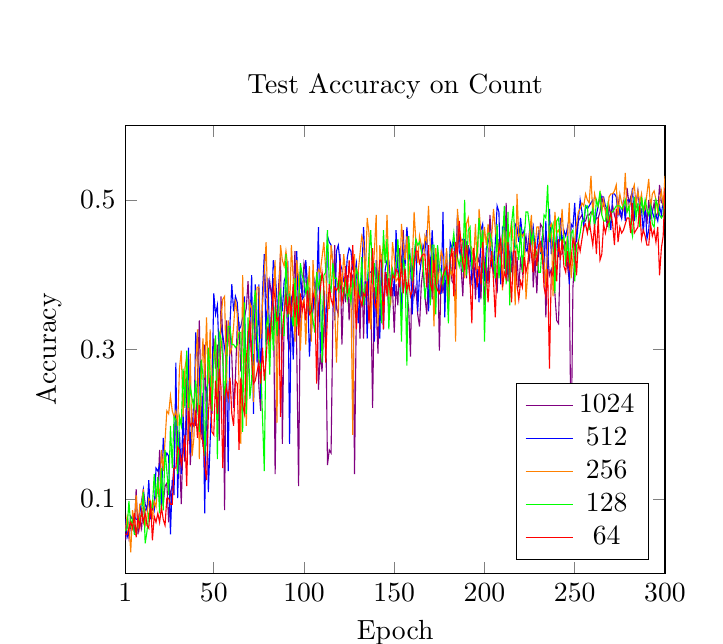
\begin{tikzpicture}
        \begin{axis}[
            title={Test Accuracy on Count},
            xlabel={Epoch},
            ylabel={Accuracy},
            xmin=1, xmax=300,
            ymin=0, ymax=0.6,
            xtick={1,50,100,150,200,250,300},
            ytick={0.1,0.3,0.5},
            legend pos=south east,
            %ymajorgrids=true,
            %grid style=dashed,
        ]

        \addplot[color=violet]
            coordinates{
                (1, 0.04435483738780022) (2, 0.07258064299821854) (3, 0.04838709533214569) (4, 0.06451612710952759) (5, 0.06451612710952759) (6, 0.05645161122083664) (7, 0.11290322989225388) (8, 0.052419353276491165) (9, 0.07258064299821854) (10, 0.06048387289047241) (11, 0.08870967477560043) (12, 0.08467742055654526) (13, 0.08870967477560043) (14, 0.09677419066429138) (15, 0.08467742055654526) (16, 0.08467742055654526) (17, 0.09677419066429138) (18, 0.10483870655298233) (19, 0.1088709682226181) (20, 0.16532258689403534) (21, 0.11693548411130905) (22, 0.0927419364452362) (23, 0.11693548411130905) (24, 0.12096773833036423) (25, 0.06854838877916336) (26, 0.1088709682226181) (27, 0.11693548411130905) (28, 0.14516128599643707) (29, 0.22580644488334656) (30, 0.17741934955120087) (31, 0.1572580635547638) (32, 0.0927419364452362) (33, 0.18145161867141724) (34, 0.14919355511665344) (35, 0.25806450843811035) (36, 0.24596774578094482) (37, 0.14516128599643707) (38, 0.19354838132858276) (39, 0.2338709682226181) (40, 0.19758065044879913) (41, 0.2620967626571655) (42, 0.33870968222618103) (43, 0.22580644488334656) (44, 0.16935484111309052) (45, 0.30645161867141724) (46, 0.2016129046678543) (47, 0.28629031777381897) (48, 0.2338709682226181) (49, 0.21370968222618103) (50, 0.3145161271095276) (51, 0.27419355511665344) (52, 0.30645161867141724) (53, 0.17741934955120087) (54, 0.3709677457809448) (55, 0.3145161271095276) (56, 0.08467742055654526) (57, 0.33870968222618103) (58, 0.3104838728904724) (59, 0.3306451737880707) (60, 0.29032257199287415) (61, 0.22177419066429138) (62, 0.2620967626571655) (63, 0.3306451737880707) (64, 0.33467742800712585) (65, 0.27016130089759827) (66, 0.3266128897666931) (67, 0.3427419364452362) (68, 0.35483869910240173) (69, 0.3911290466785431) (70, 0.33467742800712585) (71, 0.28629031777381897) (72, 0.3588709831237793) (73, 0.3145161271095276) (74, 0.32258063554763794) (75, 0.25) (76, 0.2177419364452362) (77, 0.36693549156188965) (78, 0.4072580635547638) (79, 0.3709677457809448) (80, 0.36693549156188965) (81, 0.3911290168762207) (82, 0.3709677457809448) (83, 0.39516130089759827) (84, 0.13306452333927155) (85, 0.30645161867141724) (86, 0.3870967626571655) (87, 0.42741936445236206) (88, 0.1733870953321457) (89, 0.3427419364452362) (90, 0.38306450843811035) (91, 0.3145161271095276) (92, 0.30241936445236206) (93, 0.36693549156188965) (94, 0.3790322542190552) (95, 0.43145161867141724) (96, 0.2943548262119293) (97, 0.11693548411130905) (98, 0.3709677457809448) (99, 0.3709677457809448) (100, 0.41532257199287415) (101, 0.4032258093357086) (102, 0.35080644488334656) (103, 0.38306450843811035) (104, 0.31854838132858276) (105, 0.35483869910240173) (106, 0.36693549156188965) (107, 0.39919355511665344) (108, 0.24596774578094482) (109, 0.2943548262119293) (110, 0.27016130089759827) (111, 0.3306451737880707) (112, 0.3467741906642914) (113, 0.14516128599643707) (114, 0.16532258689403534) (115, 0.16129031777381897) (116, 0.3467741906642914) (117, 0.4395161271095276) (118, 0.35483869910240173) (119, 0.3467741906642914) (120, 0.42741936445236206) (121, 0.30645161867141724) (122, 0.38306450843811035) (123, 0.3629032373428345) (124, 0.39919355511665344) (125, 0.33870968222618103) (126, 0.39516130089759827) (127, 0.39919355511665344) (128, 0.13306452333927155) (129, 0.35483869910240173) (130, 0.4072580635547638) (131, 0.3145161271095276) (132, 0.41532257199287415) (133, 0.3145161271095276) (134, 0.4072580635547638) (135, 0.3427419364452362) (136, 0.33870968222618103) (137, 0.3790322542190552) (138, 0.22177419066429138) (139, 0.38306450843811035) (140, 0.35483869910240173) (141, 0.2943548262119293) (142, 0.41532257199287415) (143, 0.4233871102333069) (144, 0.3588709533214569) (145, 0.38306450843811035) (146, 0.4032258093357086) (147, 0.33870968222618103) (148, 0.36693549156188965) (149, 0.38306450843811035) (150, 0.32258063554763794) (151, 0.3870967626571655) (152, 0.3588709831237793) (153, 0.4354838728904724) (154, 0.41129031777381897) (155, 0.45967742800712585) (156, 0.38306450843811035) (157, 0.375) (158, 0.35483869910240173) (159, 0.29032257199287415) (160, 0.4354838728904724) (161, 0.3709677457809448) (162, 0.38306450843811035) (163, 0.3467741906642914) (164, 0.3306451737880707) (165, 0.3870967626571655) (166, 0.4072580635547638) (167, 0.3709677457809448) (168, 0.3467741906642914) (169, 0.39919355511665344) (170, 0.4233871102333069) (171, 0.36693549156188965) (172, 0.3870967626571655) (173, 0.3629032373428345) (174, 0.4354838728904724) (175, 0.2983871102333069) (176, 0.4032258093357086) (177, 0.375) (178, 0.4072580635547638) (179, 0.39919355511665344) (180, 0.3588709533214569) (181, 0.4233871102333069) (182, 0.3911290466785431) (183, 0.3870967626571655) (184, 0.36693549156188965) (185, 0.4516128897666931) (186, 0.45967742800712585) (187, 0.41129031777381897) (188, 0.3709677457809448) (189, 0.44758063554763794) (190, 0.39516130089759827) (191, 0.4395161271095276) (192, 0.3870967626571655) (193, 0.4032258093357086) (194, 0.42741936445236206) (195, 0.36693549156188965) (196, 0.41532257199287415) (197, 0.4233871102333069) (198, 0.36693549156188965) (199, 0.42741936445236206) (200, 0.3588709533214569) (201, 0.41532257199287415) (202, 0.3870967626571655) (203, 0.47983869910240173) (204, 0.44758063554763794) (205, 0.41532257199287415) (206, 0.39516130089759827) (207, 0.375) (208, 0.44758063554763794) (209, 0.4193548262119293) (210, 0.44354838132858276) (211, 0.4072580635547638) (212, 0.4959677457809448) (213, 0.3911290168762207) (214, 0.43145161867141724) (215, 0.4032258093357086) (216, 0.43145161867141724) (217, 0.3709677457809448) (218, 0.4233871102333069) (219, 0.38306450843811035) (220, 0.4193548262119293) (221, 0.4032258093357086) (222, 0.4395161271095276) (223, 0.4516128897666931) (224, 0.43145161867141724) (225, 0.4193548262119293) (226, 0.4717741906642914) (227, 0.38306450843811035) (228, 0.4233871102333069) (229, 0.375) (230, 0.43145161867141724) (231, 0.4677419364452362) (232, 0.46370968222618103) (233, 0.44354838132858276) (234, 0.3427419364452362) (235, 0.42741936445236206) (236, 0.39919355511665344) (237, 0.4072580635547638) (238, 0.3911290466785431) (239, 0.375) (240, 0.33870968222618103) (241, 0.33467742800712585) (242, 0.42741936445236206) (243, 0.42741936445236206) (244, 0.4395161271095276) (245, 0.44354838132858276) (246, 0.41129031777381897) (247, 0.3911290466785431) (248, 0.16129031777381897) (249, 0.38306450843811035) (250, 0.4233871102333069) (251, 0.45967742800712585) (252, 0.4717741906642914) (253, 0.47580644488334656) (254, 0.47983869910240173) (255, 0.4717741906642914) (256, 0.4717741906642914) (257, 0.47983869910240173) (258, 0.47983869910240173) (259, 0.4838709831237793) (260, 0.4838709831237793) (261, 0.4677419364452362) (262, 0.47580644488334656) (263, 0.47580644488334656) (264, 0.4838709831237793) (265, 0.5040322542190552) (266, 0.49193549156188965) (267, 0.4879032373428345) (268, 0.46370968222618103) (269, 0.49193549156188965) (270, 0.47983869910240173) (271, 0.49193549156188965) (272, 0.47983869910240173) (273, 0.4717741906642914) (274, 0.5) (275, 0.47983869910240173) (276, 0.47580644488334656) (277, 0.4959677457809448) (278, 0.47983869910240173) (279, 0.5161290168762207) (280, 0.4959677457809448) (281, 0.5040322542190552) (282, 0.47580644488334656) (283, 0.4879032373428345) (284, 0.49193549156188965) (285, 0.4879032373428345) (286, 0.49193549156188965) (287, 0.5) (288, 0.4838709831237793) (289, 0.4959677457809448) (290, 0.4677419364452362) (291, 0.5) (292, 0.47580644488334656) (293, 0.4838709831237793) (294, 0.4959677457809448) (295, 0.47580644488334656) (296, 0.4838709533214569) (297, 0.5201612710952759) (298, 0.4959677457809448) (299, 0.4959677457809448) (300, 0.5)
            };
            \addlegendentry{1024}

        \addplot[color=blue]
            coordinates{
                (1, 0.07258064299821854) (2, 0.04838709533214569) (3, 0.05645161122083664) (4, 0.07661290466785431) (5, 0.07258064299821854) (6, 0.07661290466785431) (7, 0.07258064299821854) (8, 0.07258064299821854) (9, 0.08064515888690948) (10, 0.09677419066429138) (11, 0.11290322244167328) (12, 0.0927419364452362) (13, 0.08467742055654526) (14, 0.125) (15, 0.07258064299821854) (16, 0.0927419364452362) (17, 0.08467742055654526) (18, 0.1411290317773819) (19, 0.13709677755832672) (20, 0.14516128599643707) (21, 0.08870967477560043) (22, 0.18145161867141724) (23, 0.15322580933570862) (24, 0.16129031777381897) (25, 0.1572580635547638) (26, 0.052419353276491165) (27, 0.125) (28, 0.10483870655298233) (29, 0.2822580635547638) (30, 0.10080645233392715) (31, 0.1895161271095276) (32, 0.13306452333927155) (33, 0.21370968222618103) (34, 0.1572580635547638) (35, 0.20564515888690948) (36, 0.30241936445236206) (37, 0.16129031777381897) (38, 0.2016129046678543) (39, 0.19758065044879913) (40, 0.32258063554763794) (41, 0.29032257199287415) (42, 0.27419355511665344) (43, 0.1854838728904724) (44, 0.24193549156188965) (45, 0.08064515888690948) (46, 0.25) (47, 0.1088709682226181) (48, 0.17741934955120087) (49, 0.24193547666072845) (50, 0.375) (51, 0.3467741906642914) (52, 0.3588709533214569) (53, 0.29032257199287415) (54, 0.3306451737880707) (55, 0.31854838132858276) (56, 0.30241936445236206) (57, 0.2822580635547638) (58, 0.13709677755832672) (59, 0.33467742800712585) (60, 0.3870967626571655) (61, 0.35080644488334656) (62, 0.3709677457809448) (63, 0.3629032373428345) (64, 0.3266128897666931) (65, 0.3306451737880707) (66, 0.3427419364452362) (67, 0.3709677457809448) (68, 0.23790322244167328) (69, 0.27016130089759827) (70, 0.3306451737880707) (71, 0.39919355511665344) (72, 0.21370968222618103) (73, 0.3870967626571655) (74, 0.2822580635547638) (75, 0.3870967626571655) (76, 0.2338709682226181) (77, 0.375) (78, 0.42741936445236206) (79, 0.30645161867141724) (80, 0.39516130089759827) (81, 0.3104838728904724) (82, 0.35483869910240173) (83, 0.4193548262119293) (84, 0.4032258093357086) (85, 0.36693549156188965) (86, 0.3104838728904724) (87, 0.375) (88, 0.35080644488334656) (89, 0.3911290168762207) (90, 0.39919355511665344) (91, 0.41129031777381897) (92, 0.1733870953321457) (93, 0.3709677457809448) (94, 0.28629031777381897) (95, 0.3467741906642914) (96, 0.43145161867141724) (97, 0.33870968222618103) (98, 0.4072580635547638) (99, 0.36693549156188965) (100, 0.3709677457809448) (101, 0.4193548262119293) (102, 0.38306450843811035) (103, 0.29032257199287415) (104, 0.33870968222618103) (105, 0.35483869910240173) (106, 0.3911290466785431) (107, 0.375) (108, 0.46370968222618103) (109, 0.2943548262119293) (110, 0.33467742800712585) (111, 0.3790322542190552) (112, 0.30645161867141724) (113, 0.4516128897666931) (114, 0.44354838132858276) (115, 0.4395161271095276) (116, 0.41532257199287415) (117, 0.33870968222618103) (118, 0.43145161867141724) (119, 0.4395161271095276) (120, 0.41532257199287415) (121, 0.4072580635547638) (122, 0.3911290466785431) (123, 0.3870967626571655) (124, 0.4233871102333069) (125, 0.4354838728904724) (126, 0.43145161867141724) (127, 0.4072580635547638) (128, 0.4032258093357086) (129, 0.41532257199287415) (130, 0.33467742800712585) (131, 0.3709677457809448) (132, 0.39919355511665344) (133, 0.46370968222618103) (134, 0.4072580635547638) (135, 0.3145161271095276) (136, 0.4032258093357086) (137, 0.4032258093357086) (138, 0.4072580635547638) (139, 0.3104838728904724) (140, 0.4193548262119293) (141, 0.3790322542190552) (142, 0.3145161271095276) (143, 0.42741936445236206) (144, 0.3266128897666931) (145, 0.4072580635547638) (146, 0.4193548262119293) (147, 0.4193548262119293) (148, 0.3870967626571655) (149, 0.39919355511665344) (150, 0.3709677457809448) (151, 0.45967742800712585) (152, 0.4072580635547638) (153, 0.39919355511665344) (154, 0.3427419364452362) (155, 0.44758063554763794) (156, 0.41129031777381897) (157, 0.46370968222618103) (158, 0.43145161867141724) (159, 0.41532257199287415) (160, 0.3467741906642914) (161, 0.41129031777381897) (162, 0.44758063554763794) (163, 0.35080644488334656) (164, 0.39919355511665344) (165, 0.4193548262119293) (166, 0.4395161271095276) (167, 0.43145161867141724) (168, 0.45967742800712585) (169, 0.35080644488334656) (170, 0.4032258093357086) (171, 0.45967742800712585) (172, 0.4072580635547638) (173, 0.42741936445236206) (174, 0.4233871102333069) (175, 0.375) (176, 0.375) (177, 0.4838709533214569) (178, 0.3427419364452362) (179, 0.43145161867141724) (180, 0.3709677457809448) (181, 0.44354838132858276) (182, 0.4354838728904724) (183, 0.44354838132858276) (184, 0.4072580635547638) (185, 0.47983869910240173) (186, 0.43145161867141724) (187, 0.4233871102333069) (188, 0.44758063554763794) (189, 0.44758063554763794) (190, 0.44354838132858276) (191, 0.4233871102333069) (192, 0.4354838728904724) (193, 0.3911290466785431) (194, 0.4072580635547638) (195, 0.3870967626571655) (196, 0.4032258093357086) (197, 0.3629032373428345) (198, 0.45967742800712585) (199, 0.4677419364452362) (200, 0.3911290466785431) (201, 0.4354838728904724) (202, 0.44354838132858276) (203, 0.4516128897666931) (204, 0.41129031777381897) (205, 0.4032258093357086) (206, 0.44354838132858276) (207, 0.49193549156188965) (208, 0.4838709533214569) (209, 0.3870967626571655) (210, 0.46370968222618103) (211, 0.46370968222618103) (212, 0.39516130089759827) (213, 0.4677419364452362) (214, 0.4032258093357086) (215, 0.42741936445236206) (216, 0.41129031777381897) (217, 0.4677419364452362) (218, 0.46370968222618103) (219, 0.44354838132858276) (220, 0.47580644488334656) (221, 0.4516128897666931) (222, 0.45967742800712585) (223, 0.43145161867141724) (224, 0.4354838728904724) (225, 0.45967742800712585) (226, 0.44758063554763794) (227, 0.46370968222618103) (228, 0.4354838728904724) (229, 0.4354838728904724) (230, 0.45967742800712585) (231, 0.42741936445236206) (232, 0.4516128897666931) (233, 0.39919355511665344) (234, 0.4717741906642914) (235, 0.39919355511665344) (236, 0.4879032373428345) (237, 0.42741936445236206) (238, 0.44758063554763794) (239, 0.42741936445236206) (240, 0.4556451737880707) (241, 0.4233871102333069) (242, 0.47580644488334656) (243, 0.4395161271095276) (244, 0.45967742800712585) (245, 0.4516128897666931) (246, 0.46370968222618103) (247, 0.3870967626571655) (248, 0.4677419364452362) (249, 0.46370968222618103) (250, 0.4959677457809448) (251, 0.44354838132858276) (252, 0.4717741906642914) (253, 0.5) (254, 0.4838709533214569) (255, 0.46370968222618103) (256, 0.49193549156188965) (257, 0.4879032373428345) (258, 0.49193549156188965) (259, 0.4959677457809448) (260, 0.5) (261, 0.4677419364452362) (262, 0.47983869910240173) (263, 0.49193549156188965) (264, 0.5040322542190552) (265, 0.5040322542190552) (266, 0.5040322542190552) (267, 0.49193549156188965) (268, 0.4879032373428345) (269, 0.47983869910240173) (270, 0.45967742800712585) (271, 0.5080645084381104) (272, 0.5080645084381104) (273, 0.5040322542190552) (274, 0.47983869910240173) (275, 0.4879032373428345) (276, 0.47580644488334656) (277, 0.5) (278, 0.4717741906642914) (279, 0.5) (280, 0.5) (281, 0.4959677457809448) (282, 0.5161290168762207) (283, 0.4717741906642914) (284, 0.4959677457809448) (285, 0.5120967626571655) (286, 0.4879032373428345) (287, 0.4879032373428345) (288, 0.4556451737880707) (289, 0.4959677457809448) (290, 0.44758063554763794) (291, 0.45967742800712585) (292, 0.4959677457809448) (293, 0.4838709533214569) (294, 0.47580644488334656) (295, 0.47983869910240173) (296, 0.4717741906642914) (297, 0.49193549156188965) (298, 0.47983869910240173) (299, 0.5) (300, 0.4879032373428345) 
            };
            \addlegendentry{512}
            
        \addplot[color=orange]
            coordinates{
                (1, 0.05645161494612694) (2, 0.07661290466785431) (3, 0.06451612710952759) (4, 0.02822580747306347) (5, 0.08467742055654526) (6, 0.06854838877916336) (7, 0.10483870655298233) (8, 0.06048387289047241) (9, 0.0927419364452362) (10, 0.0927419364452362) (11, 0.11290322244167328) (12, 0.06451612710952759) (13, 0.07661290466785431) (14, 0.10080645233392715) (15, 0.09677419066429138) (16, 0.07258064299821854) (17, 0.09677419066429138) (18, 0.08870967477560043) (19, 0.125) (20, 0.09677419066429138) (21, 0.16532258689403534) (22, 0.13709677755832672) (23, 0.17741934955120087) (24, 0.2177419364452362) (25, 0.21370968222618103) (26, 0.23790322244167328) (27, 0.2177419364452362) (28, 0.20967741310596466) (29, 0.2177419364452362) (30, 0.19758065044879913) (31, 0.27419355511665344) (32, 0.2983871102333069) (33, 0.20967741310596466) (34, 0.27419355511665344) (35, 0.29032257199287415) (36, 0.17741934955120087) (37, 0.2943548262119293) (38, 0.1572580635547638) (39, 0.18145161867141724) (40, 0.2782258093357086) (41, 0.3266128897666931) (42, 0.15322580933570862) (43, 0.25806450843811035) (44, 0.3145161271095276) (45, 0.2620967626571655) (46, 0.3427419364452362) (47, 0.2540322542190552) (48, 0.3266128897666931) (49, 0.2177419364452362) (50, 0.2943548262119293) (51, 0.3145161271095276) (52, 0.2338709682226181) (53, 0.2540322542190552) (54, 0.3427419364452362) (55, 0.36693549156188965) (56, 0.3709677457809448) (57, 0.2540322542190552) (58, 0.33870968222618103) (59, 0.2943548262119293) (60, 0.30241936445236206) (61, 0.3306451737880707) (62, 0.36693549156188965) (63, 0.3467741906642914) (64, 0.2540322542190552) (65, 0.1733870953321457) (66, 0.39919355511665344) (67, 0.30241936445236206) (68, 0.19758065044879913) (69, 0.28629031777381897) (70, 0.3629032373428345) (71, 0.35483869910240173) (72, 0.22983871400356293) (73, 0.33467742800712585) (74, 0.38306450843811035) (75, 0.38306450843811035) (76, 0.3145161271095276) (77, 0.3588709533214569) (78, 0.4032258093357086) (79, 0.44354838132858276) (80, 0.3427419364452362) (81, 0.2943548262119293) (82, 0.3467741906642914) (83, 0.36693549156188965) (84, 0.4193548262119293) (85, 0.2016129046678543) (86, 0.35483869910240173) (87, 0.4395161271095276) (88, 0.4193548262119293) (89, 0.41129031777381897) (90, 0.43145161867141724) (91, 0.41129031777381897) (92, 0.3467741906642914) (93, 0.4395161271095276) (94, 0.39516130089759827) (95, 0.3104838728904724) (96, 0.4193548262119293) (97, 0.39516130089759827) (98, 0.2983871102333069) (99, 0.3588709533214569) (100, 0.36693549156188965) (101, 0.30645161867141724) (102, 0.375) (103, 0.41129031777381897) (104, 0.3104838728904724) (105, 0.4193548262119293) (106, 0.3588709533214569) (107, 0.39516130089759827) (108, 0.4072580635547638) (109, 0.4032258093357086) (110, 0.4233871102333069) (111, 0.44354838132858276) (112, 0.4072580635547638) (113, 0.35483869910240173) (114, 0.35483869910240173) (115, 0.4395161271095276) (116, 0.41532257199287415) (117, 0.35483869910240173) (118, 0.2822580635547638) (119, 0.3588709533214569) (120, 0.41129031777381897) (121, 0.3790322542190552) (122, 0.42741936445236206) (123, 0.4032258093357086) (124, 0.375) (125, 0.3709677457809448) (126, 0.38306450843811035) (127, 0.1854838728904724) (128, 0.42741936445236206) (129, 0.35080644488334656) (130, 0.4032258093357086) (131, 0.42741936445236206) (132, 0.4516128897666931) (133, 0.44354838132858276) (134, 0.3911290466785431) (135, 0.47580644488334656) (136, 0.4556451737880707) (137, 0.3266128897666931) (138, 0.3911290168762207) (139, 0.43145161867141724) (140, 0.47983869910240173) (141, 0.3306451737880707) (142, 0.4395161271095276) (143, 0.41532257199287415) (144, 0.44354838132858276) (145, 0.41532257199287415) (146, 0.47983869910240173) (147, 0.4032258093357086) (148, 0.3588709831237793) (149, 0.44354838132858276) (150, 0.4233871102333069) (151, 0.3911290466785431) (152, 0.39516130089759827) (153, 0.3870967626571655) (154, 0.4677419364452362) (155, 0.4395161271095276) (156, 0.4193548262119293) (157, 0.4516128897666931) (158, 0.3911290466785431) (159, 0.4233871102333069) (160, 0.41532257199287415) (161, 0.4838709533214569) (162, 0.44354838132858276) (163, 0.41532257199287415) (164, 0.4516128897666931) (165, 0.4395161271095276) (166, 0.4032258093357086) (167, 0.4516128897666931) (168, 0.44354838132858276) (169, 0.49193549156188965) (170, 0.4354838728904724) (171, 0.42741936445236206) (172, 0.3306451737880707) (173, 0.4354838728904724) (174, 0.3870967626571655) (175, 0.4072580635547638) (176, 0.43145161867141724) (177, 0.4233871102333069) (178, 0.39919355511665344) (179, 0.4354838728904724) (180, 0.3588709533214569) (181, 0.4072580635547638) (182, 0.39919355511665344) (183, 0.43145161867141724) (184, 0.3104838728904724) (185, 0.4879032373428345) (186, 0.45967742800712585) (187, 0.44758063554763794) (188, 0.44354838132858276) (189, 0.39516130089759827) (190, 0.4677419364452362) (191, 0.47580644488334656) (192, 0.4395161271095276) (193, 0.4354838728904724) (194, 0.4193548262119293) (195, 0.4677419364452362) (196, 0.4072580635547638) (197, 0.4879032373428345) (198, 0.4556451737880707) (199, 0.42741936445236206) (200, 0.46370968222618103) (201, 0.4395161271095276) (202, 0.4677419364452362) (203, 0.4354838728904724) (204, 0.4516128897666931) (205, 0.4879032373428345) (206, 0.45967742800712585) (207, 0.44354838132858276) (208, 0.42741936445236206) (209, 0.4354838728904724) (210, 0.3790322542190552) (211, 0.45967742800712585) (212, 0.4354838728904724) (213, 0.45967742800712585) (214, 0.4516128897666931) (215, 0.4717741906642914) (216, 0.4395161271095276) (217, 0.3588709533214569) (218, 0.5080645084381104) (219, 0.4516128897666931) (220, 0.4556451737880707) (221, 0.4516128897666931) (222, 0.4556451737880707) (223, 0.36693549156188965) (224, 0.4032258093357086) (225, 0.4556451737880707) (226, 0.47983869910240173) (227, 0.41532257199287415) (228, 0.4354838728904724) (229, 0.46370968222618103) (230, 0.46370968222618103) (231, 0.43145161867141724) (232, 0.4354838728904724) (233, 0.4193548262119293) (234, 0.38306450843811035) (235, 0.44354838132858276) (236, 0.46370968222618103) (237, 0.4677419364452362) (238, 0.3709677457809448) (239, 0.4838709533214569) (240, 0.4556451737880707) (241, 0.45967742800712585) (242, 0.4516128897666931) (243, 0.4879032373428345) (244, 0.44354838132858276) (245, 0.43145161867141724) (246, 0.4516128897666931) (247, 0.4959677457809448) (248, 0.39516130089759827) (249, 0.4233871102333069) (250, 0.44758063554763794) (251, 0.4677419364452362) (252, 0.4838709533214569) (253, 0.4879032373428345) (254, 0.4959677457809448) (255, 0.49193549156188965) (256, 0.5080645084381104) (257, 0.5) (258, 0.4959677457809448) (259, 0.5322580933570862) (260, 0.47983869910240173) (261, 0.5080645084381104) (262, 0.4959677457809448) (263, 0.49193549156188965) (264, 0.5080645084381104) (265, 0.4838709533214569) (266, 0.5) (267, 0.4838709533214569) (268, 0.47580644488334656) (269, 0.5040322542190552) (270, 0.5080645084381104) (271, 0.5080645084381104) (272, 0.5120967626571655) (273, 0.5201612710952759) (274, 0.47983869910240173) (275, 0.5080645084381104) (276, 0.4959677457809448) (277, 0.4879032373428345) (278, 0.5362903475761414) (279, 0.4838709533214569) (280, 0.4879032373428345) (281, 0.4959677457809448) (282, 0.5120967626571655) (283, 0.5201612710952759) (284, 0.49193549156188965) (285, 0.5120967626571655) (286, 0.4959677457809448) (287, 0.5080645084381104) (288, 0.4838709533214569) (289, 0.4879032373428345) (290, 0.5080645084381104) (291, 0.5282257795333862) (292, 0.4879032373428345) (293, 0.5080645084381104) (294, 0.5120967626571655) (295, 0.5) (296, 0.4838709533214569) (297, 0.5) (298, 0.5120967626571655) (299, 0.49193549156188965) (300, 0.5322580337524414) 
            };
            \addlegendentry{256}
            
        \addplot[color=green]
            coordinates{
                (1, 0.05645161122083664) (2, 0.060483869165182114) (3, 0.09677419066429138) (4, 0.06451612710952759) (5, 0.07258064299821854) (6, 0.052419353276491165) (7, 0.052419353276491165) (8, 0.06854838877916336) (9, 0.07258064299821854) (10, 0.08064515888690948) (11, 0.1088709682226181) (12, 0.04032257944345474) (13, 0.05645161494612694) (14, 0.08064515888690948) (15, 0.08870967477560043) (16, 0.08870967477560043) (17, 0.13306452333927155) (18, 0.10080645233392715) (19, 0.12903225421905518) (20, 0.08064515888690948) (21, 0.1411290317773819) (22, 0.08467742055654526) (23, 0.16532258689403534) (24, 0.13709677755832672) (25, 0.10483870655298233) (26, 0.19758065044879913) (27, 0.1411290317773819) (28, 0.20967741310596466) (29, 0.20564515888690948) (30, 0.13306452333927155) (31, 0.20967741310596466) (32, 0.19758065044879913) (33, 0.27419355511665344) (34, 0.22177419066429138) (35, 0.2983871102333069) (36, 0.22177419066429138) (37, 0.25) (38, 0.2338709682226181) (39, 0.22177419066429138) (40, 0.25806450843811035) (41, 0.22177419066429138) (42, 0.1895161271095276) (43, 0.28629031777381897) (44, 0.2661290168762207) (45, 0.1572580635547638) (46, 0.2177419364452362) (47, 0.30241936445236206) (48, 0.2661290168762207) (49, 0.2177419364452362) (50, 0.28629031777381897) (51, 0.31854838132858276) (52, 0.15322580933570862) (53, 0.32258063554763794) (54, 0.3145161271095276) (55, 0.28629031777381897) (56, 0.22983871400356293) (57, 0.2822580635547638) (58, 0.3306451737880707) (59, 0.3306451737880707) (60, 0.30645161867141724) (61, 0.30645161867141724) (62, 0.30241936445236206) (63, 0.30645161867141724) (64, 0.32258063554763794) (65, 0.32258063554763794) (66, 0.1895161271095276) (67, 0.3629032373428345) (68, 0.21370968222618103) (69, 0.3427419364452362) (70, 0.2338709682226181) (71, 0.25806450843811035) (72, 0.35483869910240173) (73, 0.3790322542190552) (74, 0.32258063554763794) (75, 0.28629031777381897) (76, 0.2782258093357086) (77, 0.20967741310596466) (78, 0.13709677755832672) (79, 0.3306451737880707) (80, 0.3427419364452362) (81, 0.2661290168762207) (82, 0.35080644488334656) (83, 0.2983871102333069) (84, 0.3588709533214569) (85, 0.31854838132858276) (86, 0.3709677457809448) (87, 0.3790322542190552) (88, 0.31854838132858276) (89, 0.31854838132858276) (90, 0.42741936445236206) (91, 0.3427419364452362) (92, 0.375) (93, 0.3467741906642914) (94, 0.3306451737880707) (95, 0.39516130089759827) (96, 0.3306451737880707) (97, 0.35483869910240173) (98, 0.41532257199287415) (99, 0.39919355511665344) (100, 0.3911290466785431) (101, 0.375) (102, 0.3911290466785431) (103, 0.35080644488334656) (104, 0.3588709533214569) (105, 0.33870968222618103) (106, 0.32258063554763794) (107, 0.4032258093357086) (108, 0.38306450843811035) (109, 0.39516130089759827) (110, 0.2822580635547638) (111, 0.39919355511665344) (112, 0.4032258093357086) (113, 0.45967742800712585) (114, 0.3870967626571655) (115, 0.3790322542190552) (116, 0.41532257199287415) (117, 0.39516130089759827) (118, 0.39516130089759827) (119, 0.3790322542190552) (120, 0.3911290466785431) (121, 0.38306450843811035) (122, 0.3709677457809448) (123, 0.39516130089759827) (124, 0.36693549156188965) (125, 0.38306450843811035) (126, 0.3629032373428345) (127, 0.3911290466785431) (128, 0.3790322542190552) (129, 0.4072580635547638) (130, 0.39919355511665344) (131, 0.3709677457809448) (132, 0.4233871102333069) (133, 0.3588709831237793) (134, 0.3870967626571655) (135, 0.3870967626571655) (136, 0.42741936445236206) (137, 0.45967742800712585) (138, 0.3870967626571655) (139, 0.41532257199287415) (140, 0.36693549156188965) (141, 0.4032258093357086) (142, 0.39516130089759827) (143, 0.33467742800712585) (144, 0.45967742800712585) (145, 0.41532257199287415) (146, 0.44758063554763794) (147, 0.3266128897666931) (148, 0.3911290466785431) (149, 0.4072580635547638) (150, 0.39516130089759827) (151, 0.39919355511665344) (152, 0.44758063554763794) (153, 0.4032258093357086) (154, 0.3104838728904724) (155, 0.4193548262119293) (156, 0.4072580635547638) (157, 0.2782258093357086) (158, 0.4516128897666931) (159, 0.4193548262119293) (160, 0.3911290466785431) (161, 0.42741936445236206) (162, 0.44758063554763794) (163, 0.4395161271095276) (164, 0.44354838132858276) (165, 0.43145161867141724) (166, 0.4193548262119293) (167, 0.36693549156188965) (168, 0.3911290168762207) (169, 0.43145161867141724) (170, 0.3588709533214569) (171, 0.4395161271095276) (172, 0.4395161271095276) (173, 0.3467741906642914) (174, 0.4395161271095276) (175, 0.41129031777381897) (176, 0.4032258093357086) (177, 0.3870967626571655) (178, 0.4072580635547638) (179, 0.39516130089759827) (180, 0.33467742800712585) (181, 0.43145161867141724) (182, 0.4354838728904724) (183, 0.4556451737880707) (184, 0.42741936445236206) (185, 0.4233871102333069) (186, 0.41129031777381897) (187, 0.42741936445236206) (188, 0.4032258093357086) (189, 0.5) (190, 0.39919355511665344) (191, 0.45967742800712585) (192, 0.46370968222618103) (193, 0.41129031777381897) (194, 0.4233871102333069) (195, 0.4193548262119293) (196, 0.43145161867141724) (197, 0.47580644488334656) (198, 0.4354838728904724) (199, 0.45967742800712585) (200, 0.3104838728904724) (201, 0.41532257199287415) (202, 0.4556451737880707) (203, 0.4556451737880707) (204, 0.44354838132858276) (205, 0.41532257199287415) (206, 0.39516130089759827) (207, 0.4677419364452362) (208, 0.39516130089759827) (209, 0.4193548262119293) (210, 0.44758063554763794) (211, 0.49193549156188965) (212, 0.3870967626571655) (213, 0.4838709533214569) (214, 0.3588709533214569) (215, 0.4677419364452362) (216, 0.49193549156188965) (217, 0.4354838728904724) (218, 0.4395161271095276) (219, 0.4193548262119293) (220, 0.46370968222618103) (221, 0.4032258093357086) (222, 0.44758063554763794) (223, 0.4838709533214569) (224, 0.4838709831237793) (225, 0.46370968222618103) (226, 0.44354838132858276) (227, 0.4556451737880707) (228, 0.4233871102333069) (229, 0.43145161867141724) (230, 0.4032258093357086) (231, 0.4032258093357086) (232, 0.44354838132858276) (233, 0.47983869910240173) (234, 0.47580644488334656) (235, 0.5201612710952759) (236, 0.44354838132858276) (237, 0.45967742800712585) (238, 0.4677419364452362) (239, 0.375) (240, 0.4717741906642914) (241, 0.47580644488334656) (242, 0.44758063554763794) (243, 0.44354838132858276) (244, 0.4516128897666931) (245, 0.41129031777381897) (246, 0.4516128897666931) (247, 0.41129031777381897) (248, 0.4556451737880707) (249, 0.45967742800712585) (250, 0.3911290168762207) (251, 0.4395161271095276) (252, 0.44354838132858276) (253, 0.4556451737880707) (254, 0.4717741906642914) (255, 0.4717741906642914) (256, 0.49193549156188965) (257, 0.49193549156188965) (258, 0.45967742800712585) (259, 0.47983869910240173) (260, 0.4879032373428345) (261, 0.46370968222618103) (262, 0.5) (263, 0.49193549156188965) (264, 0.5120967626571655) (265, 0.47983869910240173) (266, 0.4717741906642914) (267, 0.4717741906642914) (268, 0.49193549156188965) (269, 0.46370968222618103) (270, 0.4838709831237793) (271, 0.4838709831237793) (272, 0.4879032373428345) (273, 0.49193549156188965) (274, 0.49193549156188965) (275, 0.49193549156188965) (276, 0.4879032373428345) (277, 0.49193549156188965) (278, 0.5) (279, 0.4838709533214569) (280, 0.49193549156188965) (281, 0.46370968222618103) (282, 0.4516128897666931) (283, 0.5040322542190552) (284, 0.47580644488334656) (285, 0.4959677457809448) (286, 0.46370968222618103) (287, 0.5040322542190552) (288, 0.4838709831237793) (289, 0.5) (290, 0.4879032373428345) (291, 0.47983869910240173) (292, 0.49193549156188965) (293, 0.4677419364452362) (294, 0.46370968222618103) (295, 0.5) (296, 0.49193549156188965) (297, 0.47983869910240173) (298, 0.47580644488334656) (299, 0.47983869910240173) (300, 0.5120967626571655) 
            };
            \addlegendentry{128}
        
        \addplot[color=red]
            coordinates{
                (1, 0.052419353276491165) (2, 0.052419353276491165) (3, 0.06048387289047241) (4, 0.06854838877916336) (5, 0.06048387289047241) (6, 0.08064515888690948) (7, 0.04838709533214569) (8, 0.07661290466785431) (9, 0.06048387289047241) (10, 0.08467742055654526) (11, 0.06854838877916336) (12, 0.08064515888690948) (13, 0.06451612710952759) (14, 0.06048387289047241) (15, 0.09677419066429138) (16, 0.04435483738780022) (17, 0.07661290466785431) (18, 0.06854838877916336) (19, 0.08064515888690948) (20, 0.06854838877916336) (21, 0.08870967477560043) (22, 0.07258064299821854) (23, 0.06451612710952759) (24, 0.10080645233392715) (25, 0.10080645233392715) (26, 0.0927419364452362) (27, 0.0927419364452362) (28, 0.1411290317773819) (29, 0.1411290317773819) (30, 0.16935484111309052) (31, 0.16532258689403534) (32, 0.14516128599643707) (33, 0.16129031777381897) (34, 0.1854838728904724) (35, 0.11693548411130905) (36, 0.2177419364452362) (37, 0.19758065044879913) (38, 0.2016129046678543) (39, 0.19758065044879913) (40, 0.21370968222618103) (41, 0.18145161867141724) (42, 0.22580644488334656) (43, 0.18145161867141724) (44, 0.17741934955120087) (45, 0.14516128599643707) (46, 0.125) (47, 0.21370968222618103) (48, 0.25) (49, 0.1895161271095276) (50, 0.1854838728904724) (51, 0.25806450843811035) (52, 0.21370968222618103) (53, 0.27419355511665344) (54, 0.25) (55, 0.1411290317773819) (56, 0.2338709682226181) (57, 0.25) (58, 0.2338709682226181) (59, 0.2620967626571655) (60, 0.21370968222618103) (61, 0.19758065044879913) (62, 0.25806450843811035) (63, 0.2540322542190552) (64, 0.16532258689403534) (65, 0.2620967626571655) (66, 0.22580644488334656) (67, 0.21370968222618103) (68, 0.28629031777381897) (69, 0.3145161271095276) (70, 0.33870968222618103) (71, 0.28629031777381897) (72, 0.2540322542190552) (73, 0.25806450843811035) (74, 0.27016130089759827) (75, 0.2822580635547638) (76, 0.2540322542190552) (77, 0.30241936445236206) (78, 0.25806450843811035) (79, 0.28629031777381897) (80, 0.3306451737880707) (81, 0.3104838728904724) (82, 0.3427419364452362) (83, 0.38306450843811035) (84, 0.36693549156188965) (85, 0.33870968222618103) (86, 0.3427419364452362) (87, 0.20967741310596466) (88, 0.32258063554763794) (89, 0.35080644488334656) (90, 0.3709677457809448) (91, 0.3467741906642914) (92, 0.3709677457809448) (93, 0.3427419364452362) (94, 0.3870967626571655) (95, 0.3427419364452362) (96, 0.3709677457809448) (97, 0.31854838132858276) (98, 0.375) (99, 0.35080644488334656) (100, 0.3629032373428345) (101, 0.33870968222618103) (102, 0.3790322542190552) (103, 0.3467741906642914) (104, 0.35080644488334656) (105, 0.375) (106, 0.36693549156188965) (107, 0.2540322542190552) (108, 0.3588709533214569) (109, 0.3790322542190552) (110, 0.4032258093357086) (111, 0.38306450843811035) (112, 0.2822580635547638) (113, 0.3467741906642914) (114, 0.3870967626571655) (115, 0.36693549156188965) (116, 0.3588709533214569) (117, 0.38306450843811035) (118, 0.3790322542190552) (119, 0.38306450843811035) (120, 0.4193548262119293) (121, 0.3629032373428345) (122, 0.375) (123, 0.41129031777381897) (124, 0.375) (125, 0.4193548262119293) (126, 0.38306450843811035) (127, 0.4395161271095276) (128, 0.3790322542190552) (129, 0.3266128897666931) (130, 0.375) (131, 0.36693549156188965) (132, 0.3588709533214569) (133, 0.375) (134, 0.3709677457809448) (135, 0.3911290466785431) (136, 0.33467742800712585) (137, 0.375) (138, 0.4354838728904724) (139, 0.3629032373428345) (140, 0.35483869910240173) (141, 0.3870967626571655) (142, 0.4193548262119293) (143, 0.4193548262119293) (144, 0.3266128897666931) (145, 0.4032258093357086) (146, 0.3709677457809448) (147, 0.39516130089759827) (148, 0.3709677457809448) (149, 0.39919355511665344) (150, 0.39516130089759827) (151, 0.4072580635547638) (152, 0.4032258093357086) (153, 0.38306450843811035) (154, 0.41532257199287415) (155, 0.375) (156, 0.4072580635547638) (157, 0.3790322542190552) (158, 0.3911290168762207) (159, 0.3709677457809448) (160, 0.3790322542190552) (161, 0.4072580635547638) (162, 0.43145161867141724) (163, 0.43145161867141724) (164, 0.41532257199287415) (165, 0.4233871102333069) (166, 0.42741936445236206) (167, 0.42741936445236206) (168, 0.38306450843811035) (169, 0.4395161271095276) (170, 0.3870967626571655) (171, 0.3790322542190552) (172, 0.4193548262119293) (173, 0.3870967626571655) (174, 0.3790322542190552) (175, 0.375) (176, 0.3870967626571655) (177, 0.39919355511665344) (178, 0.4072580635547638) (179, 0.41129031777381897) (180, 0.3870967626571655) (181, 0.4193548262119293) (182, 0.4354838728904724) (183, 0.3709677457809448) (184, 0.44354838132858276) (185, 0.42741936445236206) (186, 0.4717741906642914) (187, 0.4395161271095276) (188, 0.41532257199287415) (189, 0.4072580635547638) (190, 0.4395161271095276) (191, 0.4193548262119293) (192, 0.3911290168762207) (193, 0.33467742800712585) (194, 0.4354838728904724) (195, 0.41129031777381897) (196, 0.38306450843811035) (197, 0.41129031777381897) (198, 0.3870967626571655) (199, 0.44354838132858276) (200, 0.41129031777381897) (201, 0.39919355511665344) (202, 0.3629032373428345) (203, 0.4072580635547638) (204, 0.43145161867141724) (205, 0.3911290466785431) (206, 0.3427419364452362) (207, 0.41532257199287415) (208, 0.4354838728904724) (209, 0.44758063554763794) (210, 0.38306450843811035) (211, 0.4032258093357086) (212, 0.39516130089759827) (213, 0.44354838132858276) (214, 0.4072580635547638) (215, 0.3629032373428345) (216, 0.43145161867141724) (217, 0.43145161867141724) (218, 0.3870967626571655) (219, 0.36693549156188965) (220, 0.3911290466785431) (221, 0.38306450843811035) (222, 0.4233871102333069) (223, 0.4032258093357086) (224, 0.41532257199287415) (225, 0.4395161271095276) (226, 0.42741936445236206) (227, 0.4032258093357086) (228, 0.44354838132858276) (229, 0.41129031777381897) (230, 0.4395161271095276) (231, 0.44354838132858276) (232, 0.42741936445236206) (233, 0.38306450843811035) (234, 0.3709677457809448) (235, 0.4072580635547638) (236, 0.27419355511665344) (237, 0.4032258093357086) (238, 0.39919355511665344) (239, 0.44354838132858276) (240, 0.3911290466785431) (241, 0.44758063554763794) (242, 0.4193548262119293) (243, 0.44758063554763794) (244, 0.41129031777381897) (245, 0.4032258093357086) (246, 0.43145161867141724) (247, 0.4072580635547638) (248, 0.4193548262119293) (249, 0.44758063554763794) (250, 0.4395161271095276) (251, 0.39919355511665344) (252, 0.44354838132858276) (253, 0.43145161867141724) (254, 0.44758063554763794) (255, 0.46370968222618103) (256, 0.4677419364452362) (257, 0.4556451737880707) (258, 0.4717741906642914) (259, 0.4556451737880707) (260, 0.4395161271095276) (261, 0.4677419364452362) (262, 0.42741936445236206) (263, 0.47580644488334656) (264, 0.4193548262119293) (265, 0.42741936445236206) (266, 0.4677419364452362) (267, 0.4556451737880707) (268, 0.4677419364452362) (269, 0.4717741906642914) (270, 0.4838709533214569) (271, 0.4677419364452362) (272, 0.4395161271095276) (273, 0.4879032373428345) (274, 0.44354838132858276) (275, 0.46370968222618103) (276, 0.4556451737880707) (277, 0.45967742800712585) (278, 0.4677419364452362) (279, 0.47580644488334656) (280, 0.47580644488334656) (281, 0.4556451737880707) (282, 0.4959677457809448) (283, 0.4556451737880707) (284, 0.45967742800712585) (285, 0.46370968222618103) (286, 0.49193549156188965) (287, 0.44758063554763794) (288, 0.45967742800712585) (289, 0.4516128897666931) (290, 0.4395161271095276) (291, 0.4395161271095276) (292, 0.4677419364452362) (293, 0.4516128897666931) (294, 0.45967742800712585) (295, 0.44354838132858276) (296, 0.46370968222618103) (297, 0.39919355511665344) (298, 0.4354838728904724) (299, 0.4516128897666931) (300, 0.5161290168762207)
            };
            \addlegendentry{64}
        \end{axis}
    \end{tikzpicture}
    \caption{The plot shows the how the test accuracy
        varies for the dataset Count changing the number
        of hidden nodes in the LSTM.}
    \label{fig:test-accuracy-count}
\end{figure}

\begin{figure}
    \centering
    \includegraphics[width=\textwidth]{images/lstm20180708T1035_train.png}
    \caption{Confusion matrix on the training set Masks
        obtained using an LSTM of 512 hidden nodes.
        See table \ref{table:activity-dataset} for the 
        association between the number and the activity.}
    \label{fig:cm_train}
\end{figure}

\begin{figure}
    \centering
    \includegraphics[width=\textwidth]{images/lstm20180708T1035_test.png}
    \caption{Confusion matrix on the test set Masks
        obtained using an LSTM of 512 hidden nodes.
        See table \ref{table:activity-dataset} for the 
        association between the number and the activity.}
    \label{fig:cm_test}
\end{figure}

%-------------------------------------------------------------------------------

\section{Implementation}

The project has been implemented in Python using Tensorflow
and matterport/Mask-R\_CNN. Below, the list of Python files
implemented for the project with a brief description of
their behaviour.

\begin{itemize}
    \item \textbf{activity.py:} training and evaluation
        of Mask R-CNN on an extended version of COCO dataset
        that considers the dataset created on LabelBox
        during the semester.
    \item \textbf{common.py:} common information of the
        dataset that are used by multiple programs
        inside the project.
    \item \textbf{count\_zeros.py:} a tool to count the
        number of frames extracted from the video that
        do not have masks when fed to Mask R-CNN.
    \item \textbf{eval\_videos.py:} saves the confusion
        matrix using a dataset of videos and a pretrained
        model.
    \item \textbf{generate\_dataset.py:} a tool to generate
        a unique \texttt{.json} file that is later used
        when training Mask R-CNN.
    \item \textbf{generate\_npz.py:} generates the dataset
        to be fed to the LSTM for the activity recognition
        on the videos.
    \item \textbf{LSTM/extractFrames.py:} a tool to extract
        a specified number of frames from a folder
        containing videos organized in categories.
    \item \textbf{LSTM/splitDataset.py:} groups the
        videos extracted with \textbf{LSTM/ extractFrames.py}
        in a training and a test set.
    \item \textbf{mask\_video.py:} generates a video
        with the masks of the objects recognized by
        Mask R-CNN.
    \item \textbf{MaskExam.py:} a collection of functions
        used by \textbf{mask\_video.py}.
    \item \textbf{merge\_npz.py:} a tool to merge two
        consistent \texttt{.npz} files, this has been
        used to create the dataset Masks+Count.
    \item \textbf{resize\_npz.py:} a tool to resize the size
        of the frames contained in a
        \texttt{.npz} file.
    \item \textbf{split\_data.py:} generates a training and a
        test set from the \texttt{.json} file created by
        \textbf{generate\_dataset.py}.
    \item \textbf{tbevent2list.py:} a tool to get the 
        data from Tensorboard in \LaTeX\ \ format to be used
        in a \texttt{tikzpicture}.
    \item \textbf{train\_videos.py:} train the LSTM
        specifying the hyperparameters and the datasets
        to be used.
    \item \textbf{validation.py:} validate the behaviour
        of a Mask R-CNN model obtained from
        \textbf{activity.py}.
    \item \textbf{VideoClassifier.py:} implementation of
        the network containing the LSTM that it is used to
        classify videos.
    \item \textbf{videos\_to\_npz.py:} a tool to create
        \texttt{.npz} files containing the videos stored
        as a numpy array.
\end{itemize}

%-------------------------------------------------------------------------------

\section{Conclusion}

The final implementation of the LSTM managed to correctly
classify the videos by looking at their frames, achieving a
maximum accuracy on the training set of \textbf{0.928} on Masks
when using LSTM-512 and on Masks+Count when using LSTM-1024.
The highest accuracy achieved on the test set is \textbf{0.532}
on Count when using LSTM-256. Studying the plots of the
accuracy in all kind of data used, it is possible to
notice that using more than 256 hidden nodes for the LSTM 
does not improve much the performances of the network.
The reason
is due to the size of the dataset and the amount of masks
contained in it.

As previously said, the activity recognition can be improved
in multiple ways, working on both Mask R-CNN and the
extraction of the features to be used in the LSTM.
In particular, Mask R-CNN could be improved by improving
the dataset and retraining the network, while the LSTM
could be improved by feeding the data in a more accurate way.
The data could be extracted also considering the length
of the videos, that influence the temporal relation between
the frames, and the amount of pixels that compose the masks
in each frame.
Finally, since the LSTM do not consider the spatiality of the
frames, it could be replaced by a Grid LSTM, that
should be better at exploiting this kind of information.


%-------------------------------------------------------------------------------

\clearpage
\bibliography{bibliography}
\bibliographystyle{ieeetr}

%-------------------------------------------------------------------------------

\end{document}
\grid
\grid
